%==============================================================================
%  Canonical LR(1) Parser : Mini-Project Report
%  Formatting mirrors the FL house style (report class, Times, chapters).
%==============================================================================
\documentclass[11pt,a4paper]{report}

\usepackage[utf8]{inputenc}
\usepackage[T1]{fontenc}
\usepackage{mathptmx}   % Times New Roman for text and math
\usepackage[a4paper,margin=1.1in]{geometry}
\usepackage{graphicx}
\usepackage{booktabs}
\usepackage{array}
\usepackage{amsmath,amssymb}
\usepackage{float}
\usepackage{caption}
\usepackage{subcaption}
\usepackage{enumitem}
\usepackage{fancyhdr}
\usepackage{tabularx}
\usepackage{multirow}
\usepackage{xcolor}
\usepackage{listings}
\usepackage{tikz}
\usetikzlibrary{arrows.meta,positioning,fit,backgrounds,calc,automata}
\usepackage[hidelinks]{hyperref}
\usepackage{xurl}   % allow long URLs to break across lines

% --- CLASSY SPACING & TYPOGRAPHY FIXES ---
\usepackage{setspace}
\onehalfspacing

\usepackage{microtype}
\raggedbottom
\usepackage{parskip}
\setlength{\parskip}{0.5em}
% -----------------------------------------

% Clean, standard-sized headings with comfortable spacing
\usepackage{titlesec}
\titleformat{\chapter}[block]{\normalfont\Large\bfseries\centering}{Chapter \thechapter\ }{0pt}{}
\titlespacing*{\chapter}{0pt}{-20pt}{24pt}

\titleformat{\section}{\normalfont\large\bfseries}{\thesection\ }{0pt}{}
\titlespacing*{\section}{0pt}{16pt}{8pt}

\titleformat{\subsection}{\normalfont\normalsize\bfseries}{\thesubsection\ }{0pt}{}
\titlespacing*{\subsection}{0pt}{12pt}{6pt}

% Elegant Table of Contents formatting
\usepackage{tocloft}
\renewcommand{\contentsname}{Table of Contents}
\renewcommand{\cfttoctitlefont}{\hfill\Large\bfseries}
\renewcommand{\cftaftertoctitle}{\hfill}
\setlength{\cftbeforetoctitleskip}{-20pt}
\setlength{\cftaftertoctitleskip}{24pt}
\setlength{\cftbeforechapskip}{1.5ex}
\setlength{\cftbeforesecskip}{0.5ex}

% Clean captions
\captionsetup{font=small,labelfont=bf,labelsep=period}
\graphicspath{{images/}{figures/}{./}}

\renewcommand{\arraystretch}{1.3}
\newcolumntype{C}[1]{>{\centering\arraybackslash}p{#1}}
\newcolumntype{L}[1]{>{\raggedright\arraybackslash}p{#1}}
\newcolumntype{R}[1]{>{\raggedleft\arraybackslash}p{#1}}

\setlist{nosep, itemsep=0.8ex, topsep=1ex}

\pagestyle{fancy}
\fancyhf{}
\fancyfoot[C]{\thepage}
\renewcommand{\headrulewidth}{0pt}

% TikZ shared styles
\tikzset{
  block/.style={rectangle, rounded corners=2pt, draw=black!70, fill=black!4,
                align=center, minimum height=8mm, inner sep=4pt, font=\small},
  io/.style={rectangle, draw=black!70, fill=black!8, align=center,
             minimum height=8mm, inner sep=4pt, font=\small},
  flow/.style={-{Stealth[length=2mm]}, draw=black!70, thick},
}

% Listings styles ------------------------------------------------------------
\definecolor{codekw}{rgb}{0.13,0.13,0.7}
\definecolor{codecmt}{rgb}{0.0,0.5,0.0}
\definecolor{codestr}{rgb}{0.6,0.1,0.1}
\definecolor{codebg}{rgb}{0.97,0.97,0.97}

\lstdefinestyle{cpp}{
  language=C++,
  backgroundcolor=\color{codebg},
  basicstyle=\ttfamily\footnotesize,
  keywordstyle=\color{codekw}\bfseries,
  commentstyle=\color{codecmt}\itshape,
  stringstyle=\color{codestr},
  numbers=left,
  numberstyle=\tiny\color{gray},
  stepnumber=1,
  breaklines=true,
  showstringspaces=false,
  frame=single,
  tabsize=2,
  captionpos=b,
}
\lstdefinestyle{term}{
  backgroundcolor=\color{codebg},
  basicstyle=\ttfamily\scriptsize,
  breaklines=true,
  frame=single,
  columns=fullflexible,
  keepspaces=true,
}

%==============================================================================
\begin{document}
%-------------------------------- TITLE PAGE ---------------------------------
\begin{titlepage}
\begin{spacing}{1.15}
\setlength{\parskip}{0pt}
\centering

\vspace*{0.2cm}
{\Large\bfseries Kathmandu University\par}
\vspace{0.4cm}
{\large\bfseries Department of Computer Science and Engineering\par}
\vspace{0.4cm}
{\large\bfseries Dhulikhel, Kavre\par}

\vfill

% Use the real KU logo if available, otherwise draw a placeholder emblem.
\IfFileExists{kulogo.jpg}{%
  
\includegraphics[width=4cm]{kulogo.jpg}\par
}{%
  \begin{tikzpicture}[scale=0.9]
    \definecolor{kublue}{rgb}{0.08,0.16,0.47}
    \definecolor{kured}{rgb}{0.70,0.12,0.16}
    \draw[kublue, line width=1.6pt] (0,0) circle (1.6);
    \draw[kublue, line width=0.6pt] (0,0) circle (1.35);
    \draw[kublue, line width=1.2pt] (90:1.2) -- (210:1.2) -- (330:1.2) -- cycle;
    \draw[kured,  line width=1.2pt] (270:1.2) -- (30:1.2) -- (150:1.2) -- cycle;
    \node[kublue, font=\bfseries] at (0,-1.9) {KU};
  \end{tikzpicture}\par
}

\vfill

{\large\bfseries A Project Report\par}
\vspace{0.4cm}
{\large\bfseries on\par}
\vspace{0.4cm}
{\large\bfseries ``Canonical LR(1) Parser Design''\par}
\vspace{0.8cm}
{\large\bfseries [Code No: COMP 409]\par}
\vspace{0.3cm}
{\normalsize (For partial fulfillment of 4\textsuperscript{th} Year/ 1\textsuperscript{st} Semester in Computer Science / Engineering)\par}

\vfill

{\large\bfseries Submitted by:\par}
\vspace{0.3cm}
{\normalsize Prabin Aryal (08)\par}
\vspace{0.15cm}
{\normalsize Dikshit Bhatta (13)\par}
\vspace{0.15cm}
{\normalsize Tank Prasad Awasthi (10)\par}
\vspace{0.15cm}
{\normalsize Nabin Kafle (28)\par}
\vspace{0.15cm}
{\normalsize Sandesh Upadhaya (61)\par}

\vfill

{\large\bfseries Submitted to:\par}
\vspace{0.3cm}
{\normalsize Mr. Sushil Nepal\par}
\vspace{0.2cm}
{\normalsize Department of Computer Science and Engineering\par}

\vfill

{\normalsize\bfseries Submission Date: \textnormal{\today}\par}
\vspace*{0.2cm}

\end{spacing}
\end{titlepage}

%--------------------------------- ABSTRACT ----------------------------------
\pagenumbering{roman}
\chapter*{Abstract}
\addcontentsline{toc}{chapter}{Abstract}

This project explores the design and implementation of a \textbf{Canonical LR(1)
parser}, the most powerful of the deterministic bottom-up parsing techniques.
Starting from the augmented grammar
$S' \rightarrow S,\; S \rightarrow L = R \mid R,\; L \rightarrow {*}R \mid \texttt{id},\; R \rightarrow L$,
the report develops the complete theory required to build the parser: LR(1)
items, the \texttt{closure} and \texttt{goto} operations, the construction of the
canonical collection of sets of LR(1) items, and the systematic construction of
the \texttt{ACTION} and \texttt{GOTO} tables. The chosen grammar is the classic
example that is \emph{not} SLR(1)---it produces a shift/reduce conflict under
SLR---yet is conflict-free under canonical LR(1) because the items carry exact
one-symbol look-aheads. The parser is implemented in \textbf{C++}, which builds
the FIRST sets, the 14-state canonical automaton, and a conflict-free parsing
table, and then traces input strings step by step. The report demonstrates that
the table has \emph{no} conflicts and validates it on the test string
\texttt{id = *id} (accepted) while correctly rejecting the malformed string
\texttt{id = id * id}.

\medskip
\noindent\textbf{Keywords:} Bottom-up parsing, LR(1) items, Canonical LR, Shift-reduce, Parsing table, Conflict.

\vfill

%------------------------------ TABLE OF CONTENTS -----------------------------
\clearpage
\tableofcontents

%-------------------------- LIST OF FIGURES & TABLES --------------------------
\clearpage
\listoffigures
\vspace{1.5cm}
\listoftables

\cleardoublepage
\pagenumbering{arabic}

%==============================================================================
\chapter{Introduction}
%==============================================================================

\section{Background}
A \emph{parser} is the phase of a compiler that takes the stream of tokens
produced by the lexical analyzer and verifies that the tokens form a valid
sentence of the source language as described by a context-free grammar (CFG).
Parsing techniques fall into two broad families: \textbf{top-down} parsing,
which builds the parse tree from the root downwards using leftmost derivations,
and \textbf{bottom-up} parsing, which builds the tree from the leaves upwards by
reducing the input to the start symbol using reverse rightmost derivations.

\section{Bottom-up (Shift--Reduce) Parsing}
Bottom-up parsers are usually \emph{shift--reduce} parsers driven by a stack and
a parsing table. At each step the parser performs one of four actions:
\begin{itemize}
  \item \textbf{Shift} -- push the next input symbol (and the corresponding state) onto the stack;
  \item \textbf{Reduce} -- replace a handle (the right-hand side of a production) on top of the stack by the production's left-hand side;
  \item \textbf{Accept} -- the input has been successfully reduced to the start symbol;
  \item \textbf{Error} -- the configuration has no valid action.
\end{itemize}

\section{The LR Parsing Family}
\textbf{LR parsers} read input \textbf{L}eft-to-right and produce a
\textbf{R}ightmost derivation in reverse. They are table-driven and never
backtrack. The family is ordered by power:
\begin{itemize}
  \item \textbf{LR(0)} -- no look-ahead; weakest.
  \item \textbf{SLR(1)} -- LR(0) automaton with reductions restricted by FOLLOW sets.
  \item \textbf{LALR(1)} -- merges LR(1) states with identical cores; used by tools such as \texttt{yacc}/\texttt{bison}.
  \item \textbf{Canonical LR(1)} -- keeps a precise look-ahead with every item; recognizes the largest class of grammars and is the subject of this project.
\end{itemize}

\section{Why Canonical LR(1)}
The strength of canonical LR(1) is that each item carries an explicit
look-ahead terminal. This extra precision allows the parser to distinguish
situations that SLR and LR(0) merge, thereby removing spurious conflicts. The
grammar in this project is the textbook example (Aho, Lam, Sethi, Ullman) that
exposes exactly this difference: under SLR(1) it has a shift/reduce conflict,
but under canonical LR(1) it is conflict-free.

\section{Problem Statement}
Consider the following augmented grammar:
\begin{align*}
0.\quad & S' \rightarrow S \\
1.\quad & S \rightarrow L = R \\
2.\quad & S \rightarrow R \\
3.\quad & L \rightarrow {*}\,R \\
4.\quad & L \rightarrow \texttt{id} \\
5.\quad & R \rightarrow L
\end{align*}
Apply the Canonical LR parsing technique, construct the parsing table, show
that it contains \textbf{no conflict}, and test it on a string of the form
\texttt{id = id * id}.

\section{Objectives}
\begin{enumerate}
  \item To understand the theory of canonical LR(1) parsing: items, closure, goto, and table construction.
  \item To construct, by program, the canonical collection of sets of LR(1) items and the parsing table for the given grammar.
  \item To prove that the resulting table is free of shift/reduce and reduce/reduce conflicts.
  \item To implement an LR driver in C++ and validate the table on input strings, printing a complete parse trace.
\end{enumerate}

%==============================================================================
\chapter{Methodology and Theoretical Background}
%==============================================================================

\section{Augmenting the Grammar}
The first transformation is \textbf{augmentation}: a new start symbol $S'$ and a
production $S' \rightarrow S$ are added. This gives the parser a single,
unambiguous accepting production---when the parser is about to reduce by
$S' \rightarrow S$ on look-ahead \texttt{\$}, the input is accepted. Note that
this grammar requires \emph{no} other transformation: unlike top-down (LL)
parsing, LR parsing handles left recursion and common prefixes directly, so no
left-recursion removal or left factoring is needed.

\section{LR(1) Items}
An \textbf{LR(1) item} is a production with a dot ($\bullet$) marking how much of
the right-hand side has been seen, together with a one-symbol look-ahead, written
\[
[A \rightarrow \alpha \bullet \beta,\; a].
\]
The look-ahead $a$ is the terminal that is expected to follow once this
production is completed. Carrying $a$ inside the item is precisely what makes the
method ``canonical'' LR(1).

\section{The CLOSURE Operation}
For a set of items $I$, $\mathrm{CLOSURE}(I)$ adds every item that is implied by
the items already present:
\begin{quote}
For each item $[A \rightarrow \alpha \bullet B\beta,\; a]$ in $I$ and each
production $B \rightarrow \gamma$, add the item
$[B \rightarrow \bullet \gamma,\; b]$ for every terminal
$b \in \mathrm{FIRST}(\beta a)$. Repeat until no new items can be added.
\end{quote}

\section{The GOTO Operation}
$\mathrm{GOTO}(I, X)$ models the transition of the parser on a grammar symbol $X$:
\begin{quote}
$\mathrm{GOTO}(I, X) = \mathrm{CLOSURE}\big(\{\,[A \rightarrow \alpha X \bullet \beta,\; a] \mid [A \rightarrow \alpha \bullet X\beta,\; a] \in I\,\}\big).$
\end{quote}

\section{Canonical Collection of Sets of LR(1) Items}
The set of parser states is built by:
\begin{enumerate}
  \item Start with $I_0 = \mathrm{CLOSURE}(\{[S' \rightarrow \bullet S,\; \$]\})$.
  \item For each state $I$ already in the collection and each grammar symbol $X$, compute $\mathrm{GOTO}(I, X)$; if it is non-empty and new, add it as a new state.
  \item Repeat until no new states appear.
\end{enumerate}

\section{Constructing the Parsing Table}
From the canonical collection, the \texttt{ACTION} and \texttt{GOTO} tables are
filled for every state $I_i$:
\begin{itemize}
  \item If $[A \rightarrow \alpha \bullet a\beta,\; b] \in I_i$ and $a$ is a terminal with $\mathrm{GOTO}(I_i, a) = I_j$, set $\texttt{ACTION}[i, a] = \texttt{shift } j$ (written \texttt{s}$j$).
  \item If $[A \rightarrow \alpha \bullet,\; a] \in I_i$ and $A \neq S'$, set $\texttt{ACTION}[i, a] = \texttt{reduce } A \rightarrow \alpha$ (written \texttt{r}$k$).
  \item If $[S' \rightarrow S \bullet,\; \$] \in I_i$, set $\texttt{ACTION}[i, \$] = \texttt{accept}$.
  \item If $\mathrm{GOTO}(I_i, A) = I_j$ for a non-terminal $A$, set $\texttt{GOTO}[i, A] = j$.
\end{itemize}
A \textbf{conflict} occurs if any cell receives two different entries
(shift/reduce or reduce/reduce). A grammar is canonical LR(1) if and only if
this construction yields no conflicts.

\section{Key Insight: SLR Conflict vs.\ LR(1) Resolution}
This grammar is the canonical demonstration of why look-aheads matter. Computing
FOLLOW sets gives
\[
\mathrm{FOLLOW}(L) = \mathrm{FOLLOW}(R) = \{=, \$\}.
\]
The state $I_2$ contains the two items
\[
[S \rightarrow L \bullet = R,\; \$] \qquad\text{and}\qquad [R \rightarrow L \bullet,\; \$].
\]
Under \textbf{SLR(1)}, the reduce item $R \rightarrow L \bullet$ would trigger a
reduction on \emph{every} symbol of $\mathrm{FOLLOW}(R) = \{=, \$\}$. Since the
first item asks to \emph{shift} on \texttt{=}, the cell $\texttt{ACTION}[2, =]$
would hold both \texttt{shift} and \texttt{reduce}---a shift/reduce
conflict---so the grammar is \textbf{not} SLR(1).

Under \textbf{canonical LR(1)}, the look-ahead carried with
$[R \rightarrow L \bullet,\; \$]$ is exactly \texttt{\$}, \emph{not} \texttt{=}.
Therefore the reduction is placed only in $\texttt{ACTION}[2, \$]$, while the
shift stays in $\texttt{ACTION}[2, =]$. The two actions land in different cells
and \textbf{no conflict arises}. This is the precise sense in which canonical
LR(1) is stronger than SLR(1).

\section{The LR Parsing Algorithm}
The driver maintains a stack of states. Let $s$ be the state on top of the stack
and $a$ the current input symbol:
\begin{itemize}
  \item If $\texttt{ACTION}[s, a] = \texttt{s}j$: push $a$ and state $j$; advance the input.
  \item If $\texttt{ACTION}[s, a] = \texttt{r}k$ for $A \rightarrow \beta$: pop $|\beta|$ symbols/states; with $t$ now on top, push $A$ and state $\texttt{GOTO}[t, A]$.
  \item If $\texttt{ACTION}[s, a] = \texttt{accept}$: stop, input accepted.
  \item Otherwise: report a syntax error.
\end{itemize}

%==============================================================================
\chapter{Design and Implementation}
%==============================================================================

\section{Language Choice and Motivation}
The parser is implemented in \textbf{C++}. C++ was chosen because:
\begin{itemize}
  \item Its Standard Template Library (\texttt{std::set}, \texttt{std::map}, \texttt{std::vector}) maps naturally onto the mathematical objects of the algorithm---sets of items, transition maps, and ordered states---so the code reads close to the formal definitions.
  \item Ordered containers (\texttt{std::set<Item>}) give canonical, comparable representations of item sets, which makes detecting an ``already existing'' state a direct set comparison.
  \item It is compiled and fast, and is the language used throughout the compiler lab, keeping the project consistent with the rest of the coursework.
\end{itemize}

\section{Transformation Applied}
Two clarifications were required to fit the parser's constraints:
\begin{enumerate}
  \item \textbf{Augmentation.} The grammar was augmented with $S' \rightarrow S$ so that acceptance is a single, well-defined reduction. No left-recursion removal or left factoring is needed for LR parsing.
  \item \textbf{Test-string interpretation.} In this grammar \texttt{*} is a \emph{prefix} dereference operator ($L \rightarrow {*}R$, modelling an l-value such as \texttt{*p}); it never appears between two operands. Hence the well-formed reading of the requested string \texttt{id = id * id} is \texttt{id = *id} (that is, \texttt{id = * id}). The program tests both: \texttt{id = *id} is accepted, and the literal \texttt{id = id * id} is correctly rejected, which also demonstrates the parser's error detection.
\end{enumerate}

\section{System Architecture}
Figure~\ref{fig:model} shows the standard model of an LR parser. The driver is
generic; all grammar-specific knowledge lives in the parsing table.

\begin{figure}[H]
\centering
\begin{tikzpicture}[node distance=6mm and 9mm]
  \node at (0,3.2) {\textbf{Input}};
  \foreach \x/\t in {0/id,1/=,2/*,3/id,4/\$} {
    \node[io, minimum width=0.7cm] at (\x*0.75,2.6) {\t};
  }
  \node at (-3.0,0.9) {\textbf{Stack}};
  \node[io, minimum width=1cm] at (-3.0,0.2) {$X_m$};
  \node[io, minimum width=1cm] at (-3.0,-0.4) {$\vdots$};
  \node[io, minimum width=1cm] at (-3.0,-1.0) {$X_0$};
  \node[block, minimum width=2.6cm, minimum height=1cm] (drv) at (0,0) {LR Parsing\\ Driver};
  \node[block, minimum width=2.6cm, minimum height=1cm] (tab) at (0,-2.2) {ACTION / GOTO\\ Table};
  \node[block, minimum width=2.6cm, minimum height=1cm] (out) at (3.8,0) {Output\\ (derivation)};
  \draw[flow] (0.75,2.2) -- (drv.north);
  \draw[flow] (-2.3,-0.4) -- (drv.west);
  \draw[flow] (drv.west) -- (-2.3,0.0);
  \draw[{Stealth[length=2mm]}-{Stealth[length=2mm]}, draw=black!70, thick] (drv.south) -- (tab.north);
  \draw[flow] (drv.east) -- (out.west);
\end{tikzpicture}
\caption{Model of a table-driven LR parser.}
\label{fig:model}
\end{figure}

\section{Core Data Structures}
\begin{itemize}
  \item \texttt{struct Production \{ string lhs; vector<string> rhs; \}} -- one numbered grammar rule.
  \item \texttt{struct Item \{ int prod; int dot; string look; \}} -- an LR(1) item, made comparable so it can live in an ordered set.
  \item \texttt{using ItemSet = set<Item>} -- a parser state (a set of LR(1) items).
  \item \texttt{vector<ItemSet> C} -- the canonical collection of states.
  \item \texttt{map<pair<int,string>,int> TRANS} -- the goto graph of the automaton.
  \item \texttt{map<int,map<string,string>> ACTION} and \texttt{map<int,map<string,int>> GOTOT} -- the parsing table.
\end{itemize}

\section{Implementation of CLOSURE}
\begin{figure}[H]
\centering
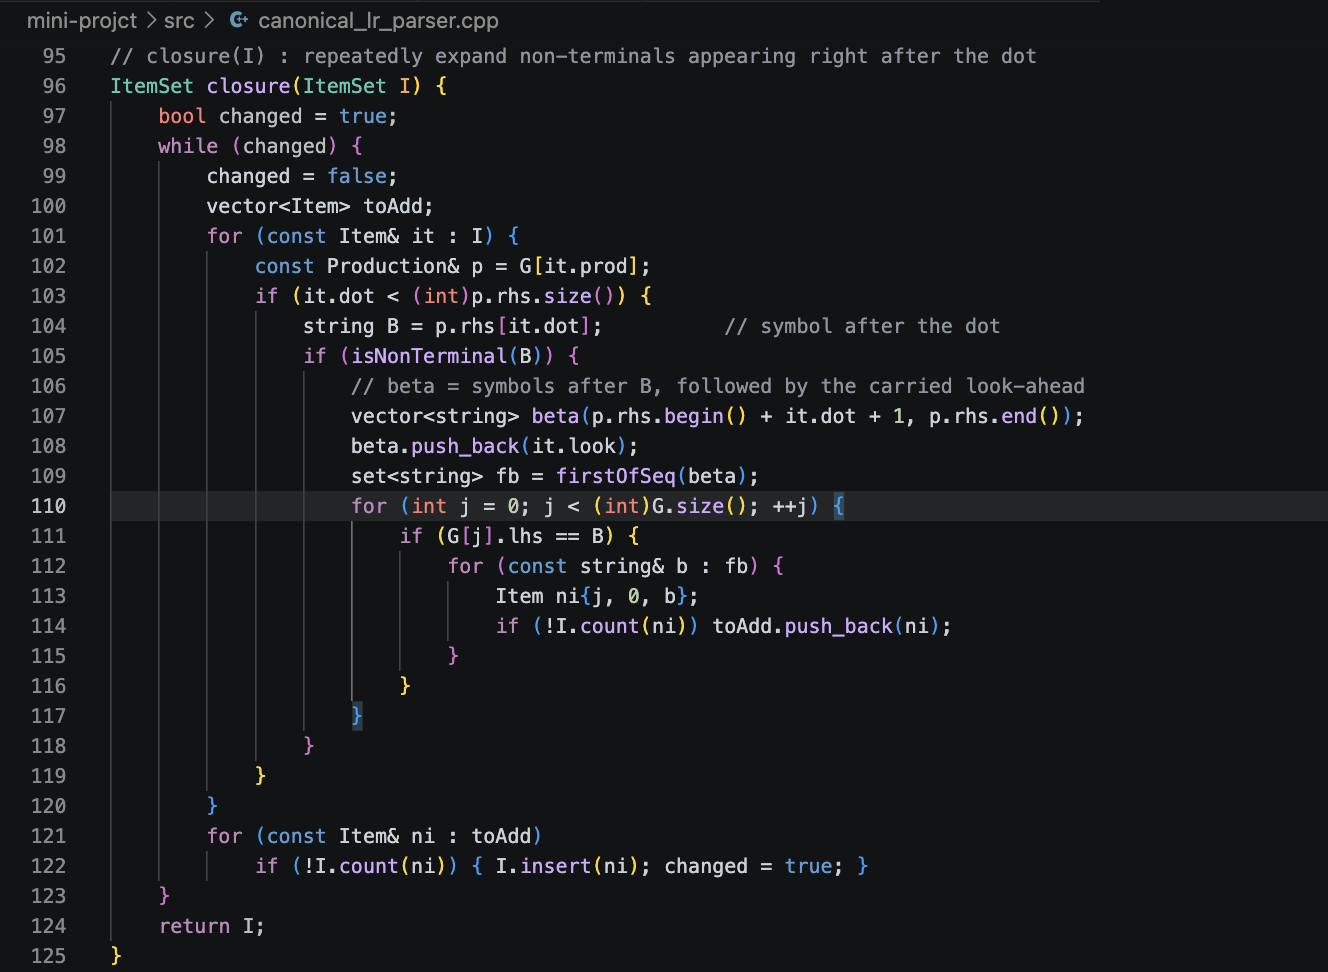
\includegraphics[width=\textwidth]{Theclosurefunction.png}
\caption{The \texttt{closure} function.}
\label{fig:closure}
\end{figure}

\section{Implementation of GOTO}
\begin{figure}[H]
\centering
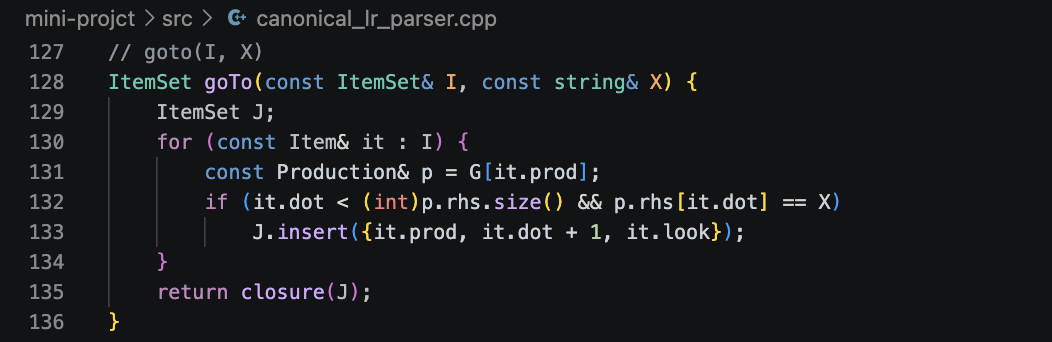
\includegraphics[width=0.95\textwidth]{thegotofunction.png}
\caption{The \texttt{goTo} function.}
\label{fig:goto-fn}
\end{figure}

\section{Building the Canonical Collection}
\begin{figure}[H]
\centering
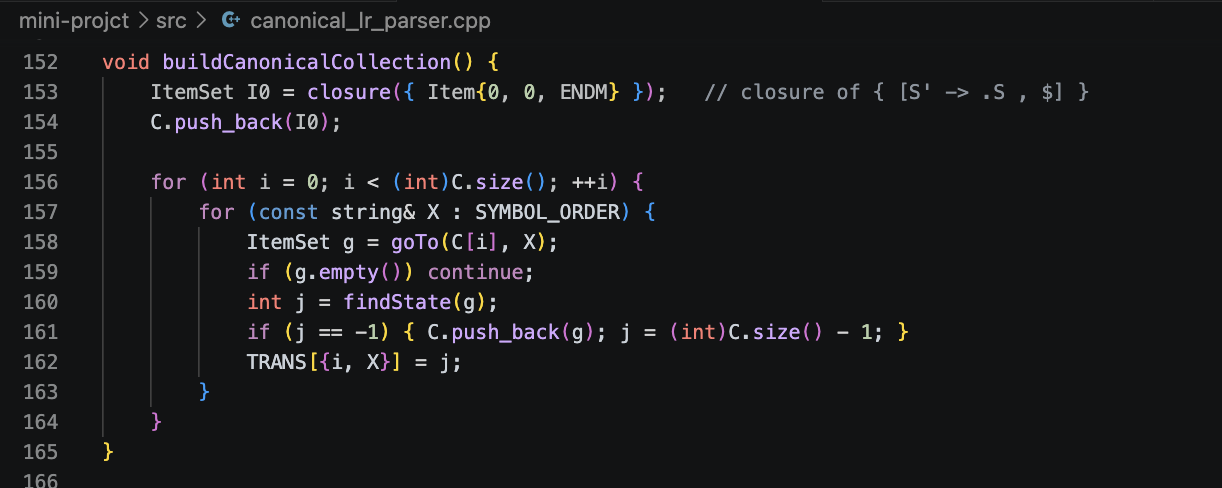
\includegraphics[width=0.95\textwidth]{buildingcanonicalcollection.png}
\caption{Building the canonical collection of LR(1) item sets.}
\label{fig:buildcc}
\end{figure}

\section{Building the Tables and Detecting Conflicts}
\begin{figure}[H]
\centering
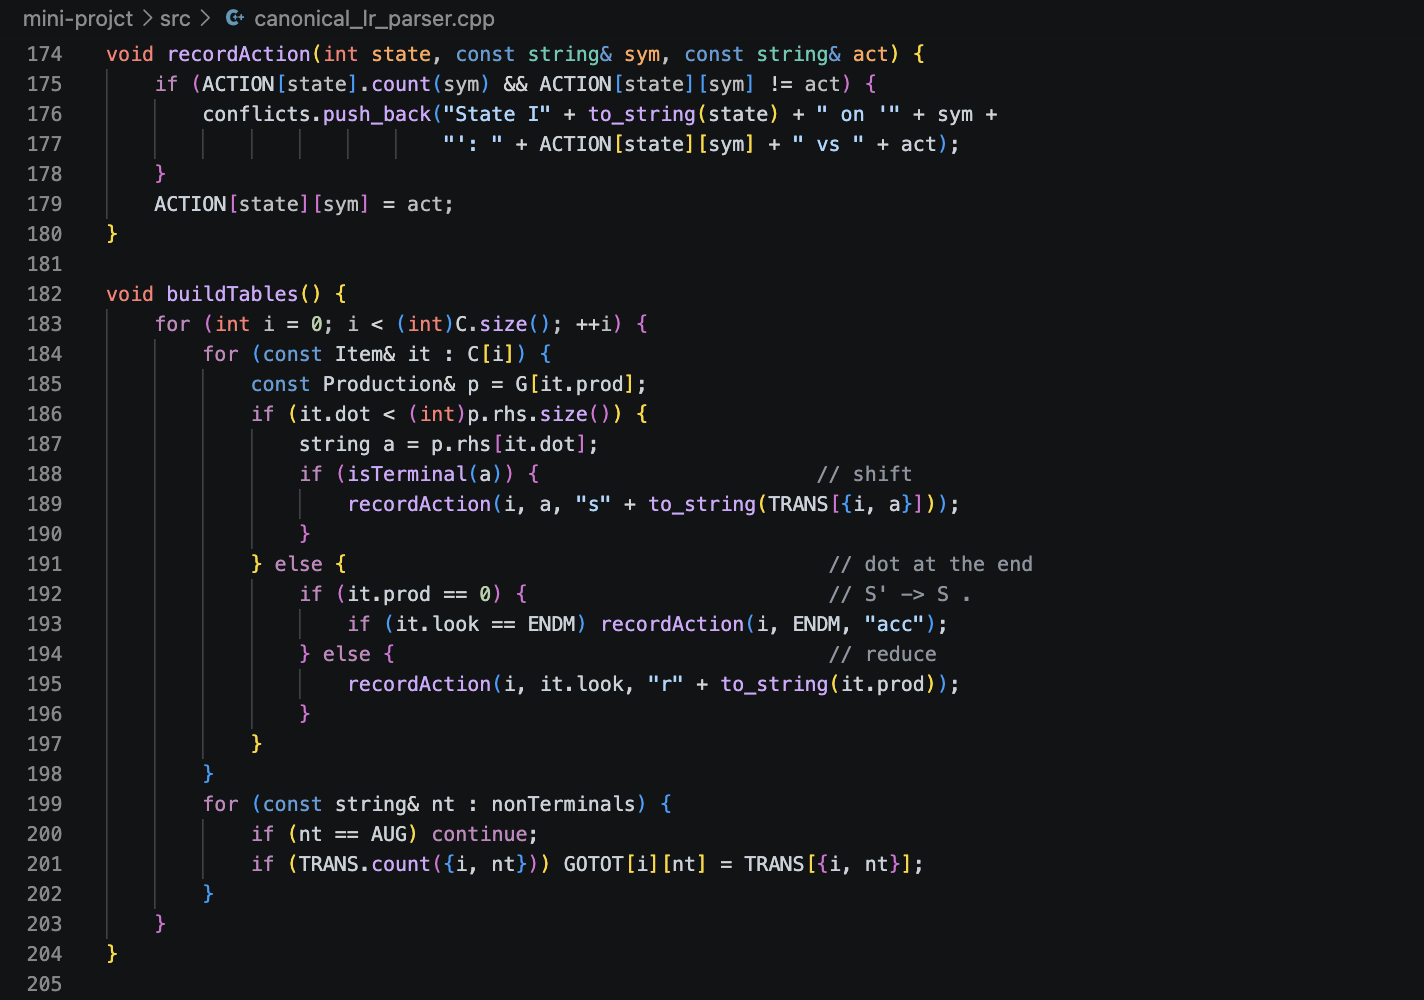
\includegraphics[width=\textwidth]{recordactionflags.png}
\caption{Filling the ACTION/GOTO tables; \texttt{recordAction} flags any conflict.}
\label{fig:buildtables}
\end{figure}

The complete source listing is given in Appendix~\ref{app:code}.

%==============================================================================
\chapter{Results}
%==============================================================================

The parser was compiled and run on macOS. The program prints its complete output
in a single run; the following screenshots show that terminal session.

\begin{figure}[H]
\centering
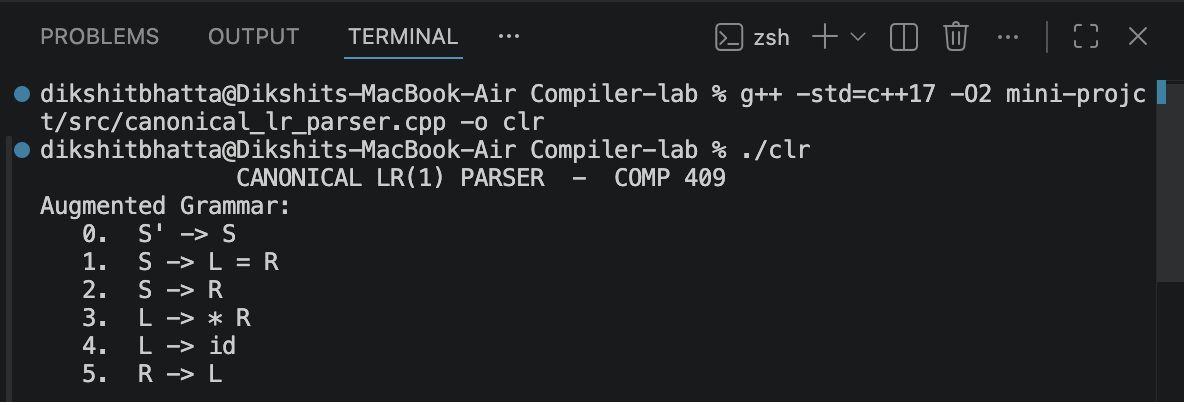
\includegraphics[width=\textwidth]{output/output1.png}
\caption{Compilation, program banner, and the augmented grammar.}
\end{figure}

\section{FIRST Sets}
\begin{figure}[H]
\centering
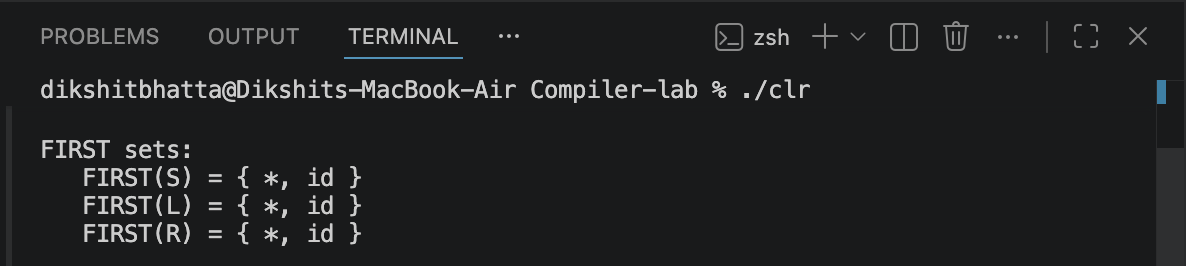
\includegraphics[width=\textwidth]{output/output2.png}
\caption{FIRST sets computed by the program.}
\end{figure}

\section{Canonical Collection of LR(1) Item Sets}
The construction produces \textbf{14 states} ($I_0 \ldots I_{13}$). Each is
listed below with its items and outgoing transitions, exactly as emitted by the
program.

\begin{figure}[H]
\centering
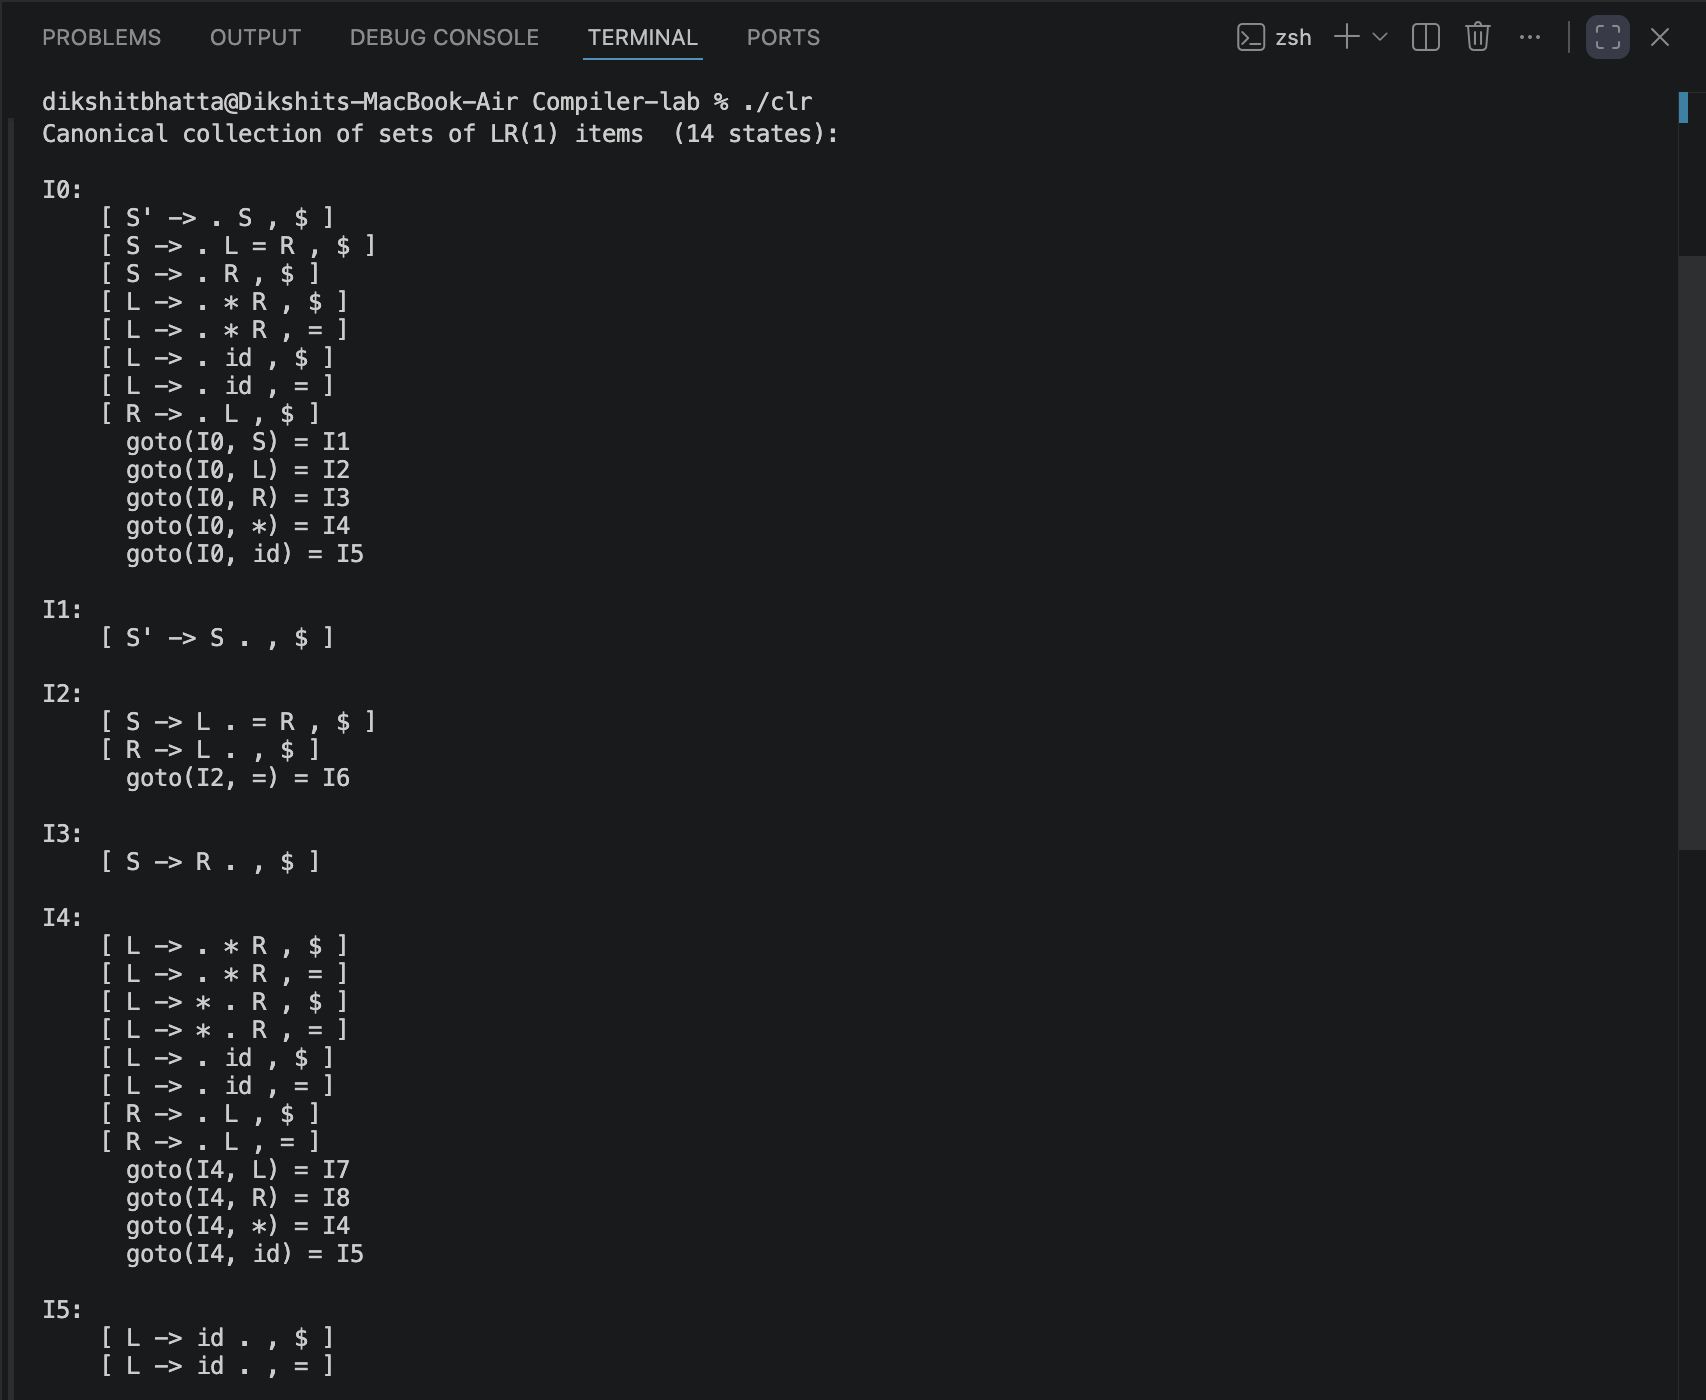
\includegraphics[width=\textwidth]{output/output3.png}
\caption{Canonical collection of LR(1) item sets: states $I_0$--$I_5$.}
\end{figure}

\begin{figure}[H]
\centering
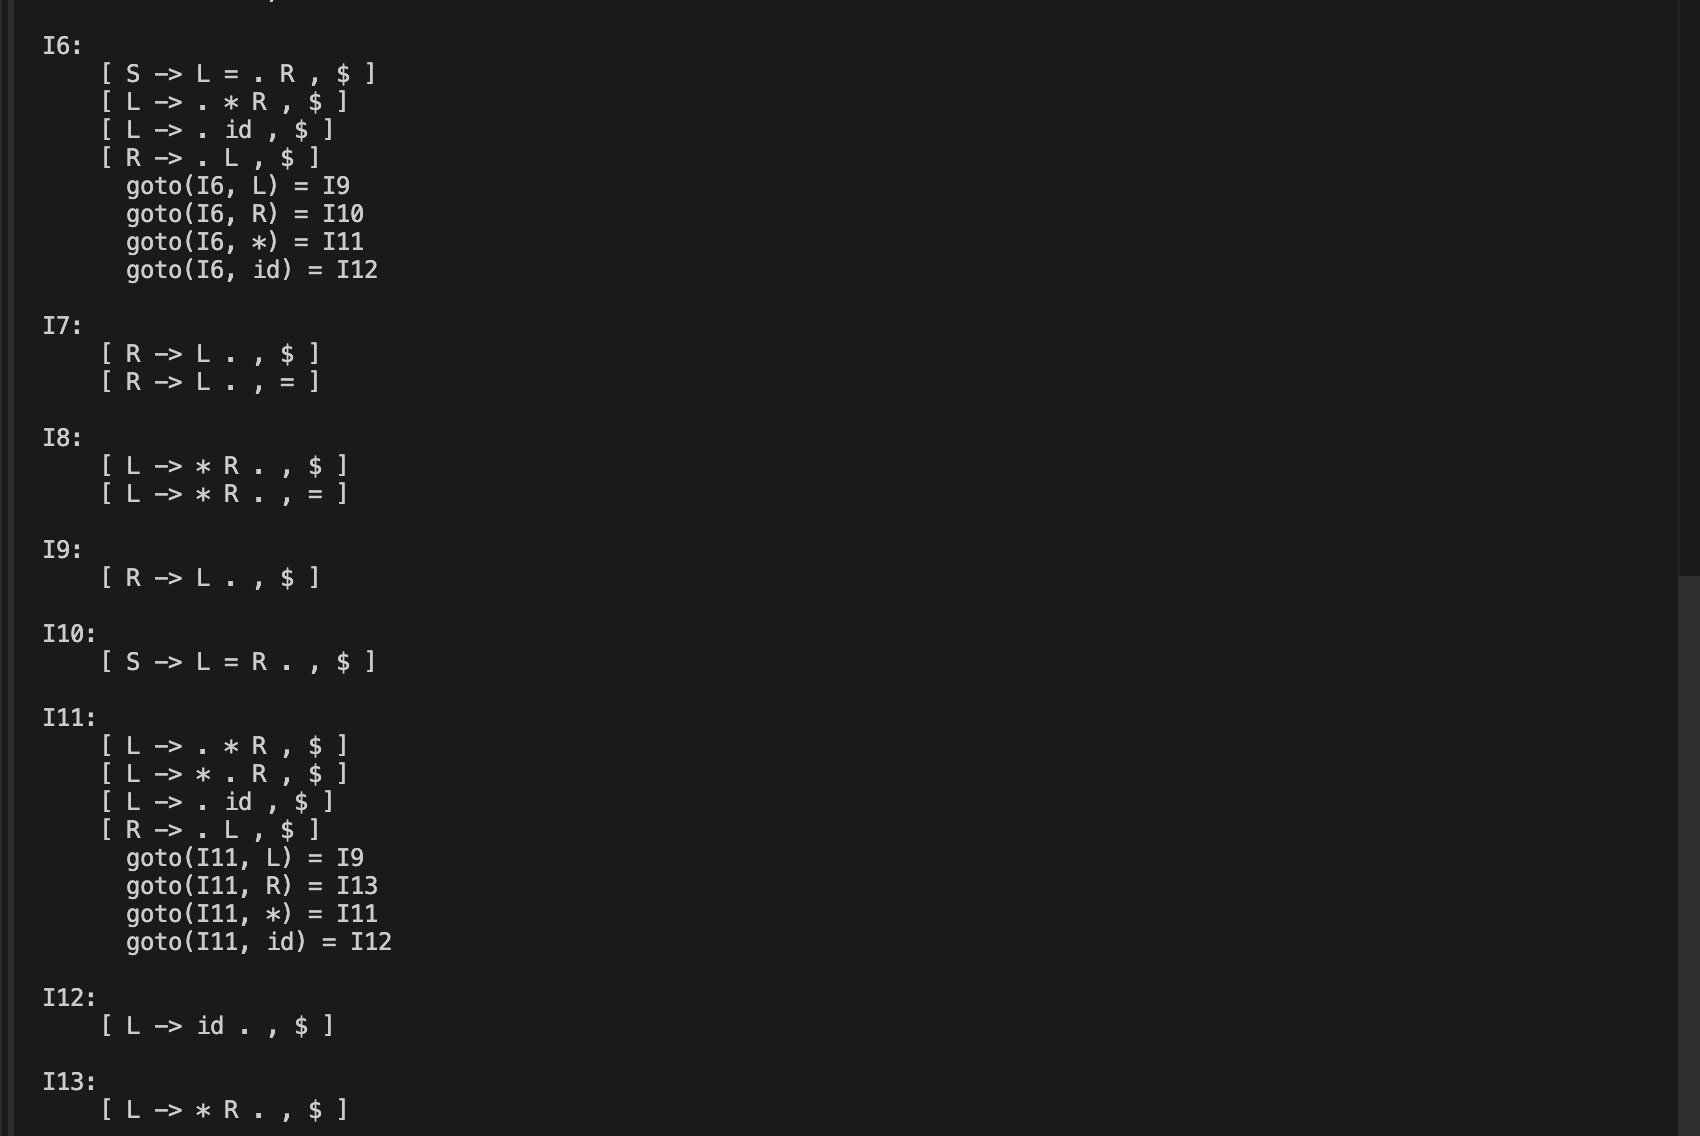
\includegraphics[width=\textwidth]{output/output4.png}
\caption{Canonical collection of LR(1) item sets: states $I_6$--$I_{13}$.}
\end{figure}

\section{Transition Diagram}
Figure~\ref{fig:goto} shows the goto graph (the DFA of viable prefixes).

\begin{figure}[H]
\centering
\begin{tikzpicture}[
  ->, >={Stealth[]}, shorten >=1pt, node distance=2.0cm and 2.4cm,
  every state/.style={draw, circle, minimum size=0.85cm, inner sep=1pt, font=\small},
  every edge/.style={draw}, auto
]
\node[state, initial, initial text=] (q0) {$I_0$};
\node[state] (q1) [above right=1.2cm and 2.4cm of q0] {$I_1$};
\node[state] (q2) [right=of q0] {$I_2$};
\node[state] (q3) [below right=0.4cm and 2.4cm of q0] {$I_3$};
\node[state] (q4) [below=3.0cm of q0] {$I_4$};
\node[state] (q5) [left=1.8cm of q4] {$I_5$};

\node[state] (q6) [right=of q2] {$I_6$};
\node[state] (q7) [below right=0.3cm and 2.0cm of q4] {$I_7$};
\node[state] (q8) [below=1.8cm of q4] {$I_8$};

\node[state] (q9)  [above right=0.2cm and 2.2cm of q6] {$I_9$};
\node[state] (q10) [right=of q6] {$I_{10}$};
\node[state] (q11) [below right=0.6cm and 2.2cm of q6] {$I_{11}$};
\node[state] (q12) [below=1.8cm of q6] {$I_{12}$};
\node[state] (q13) [right=2.4cm of q11] {$I_{13}$};

\path
 (q0) edge node {S} (q1)
 (q0) edge node {L} (q2)
 (q0) edge node[pos=0.3] {R} (q3)
 (q0) edge node[left] {*} (q4)
 (q0) edge[bend right=15] node[below left] {id} (q5)
 (q2) edge node {=} (q6)
 (q4) edge node[above] {L} (q7)
 (q4) edge node[left] {R} (q8)
 (q4) edge[loop right] node {*} (q4)
 (q4) edge node[above] {id} (q5)
 (q6) edge node[above left] {L} (q9)
 (q6) edge node {R} (q10)
 (q6) edge node[below left] {*} (q11)
 (q6) edge node[left] {id} (q12)
 (q11) edge node[left] {L} (q9)
 (q11) edge node {R} (q13)
 (q11) edge[loop below] node {*} (q11)
 (q11) edge[bend right=15] node[below] {id} (q12);
\end{tikzpicture}
\caption{Transition diagram of the canonical LR(1) automaton (14 states).}
\label{fig:goto}
\end{figure}

\section{The Parsing Table}
The canonical LR(1) parsing table produced by the program is shown in
Figure~\ref{fig:ptable} (\texttt{s}$j$ = shift to state $j$, \texttt{r}$k$ =
reduce by production $k$, \texttt{acc} = accept; blank cells are errors).

\begin{figure}[H]
\centering
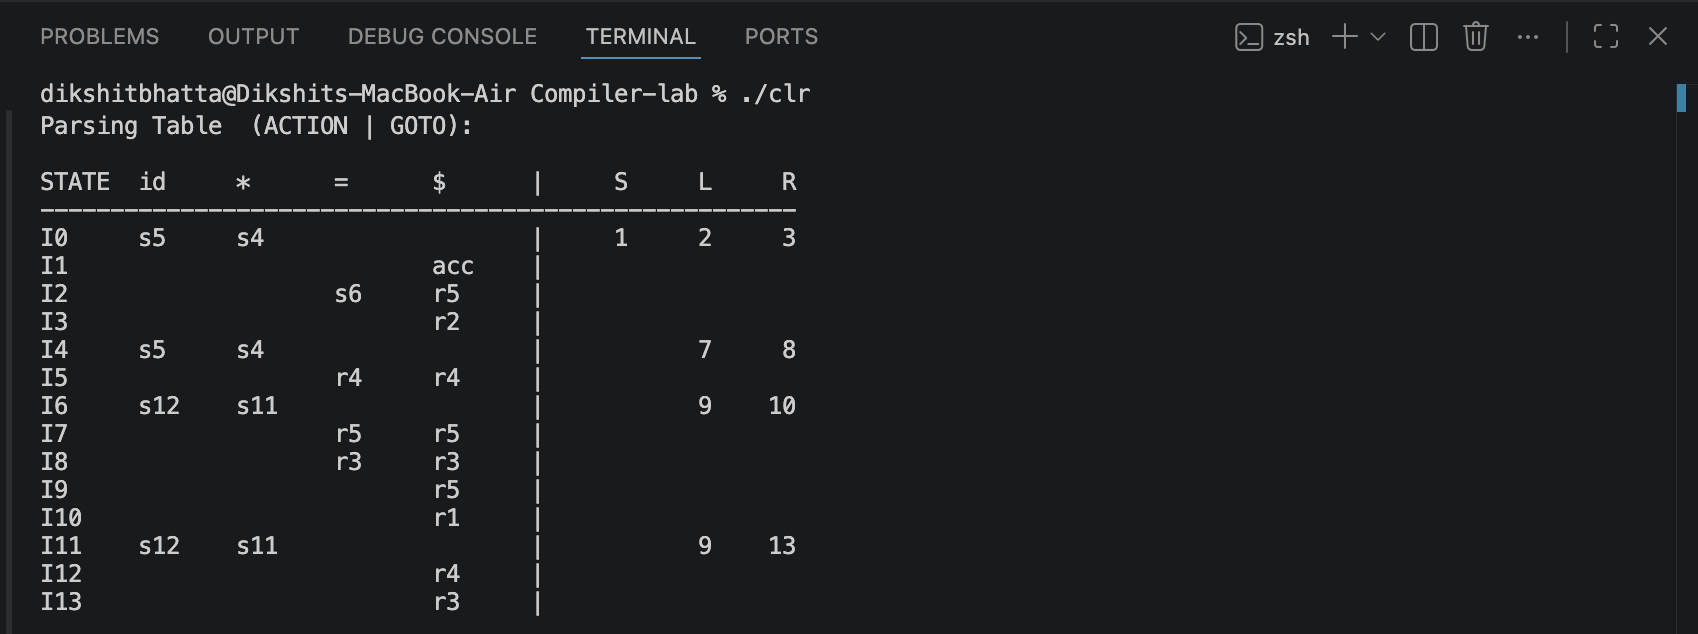
\includegraphics[width=\textwidth]{output/output5.png}
\caption{Canonical LR(1) parsing table (ACTION and GOTO).}
\label{fig:ptable}
\end{figure}

\section{Conflict Check}
\begin{figure}[H]
\centering
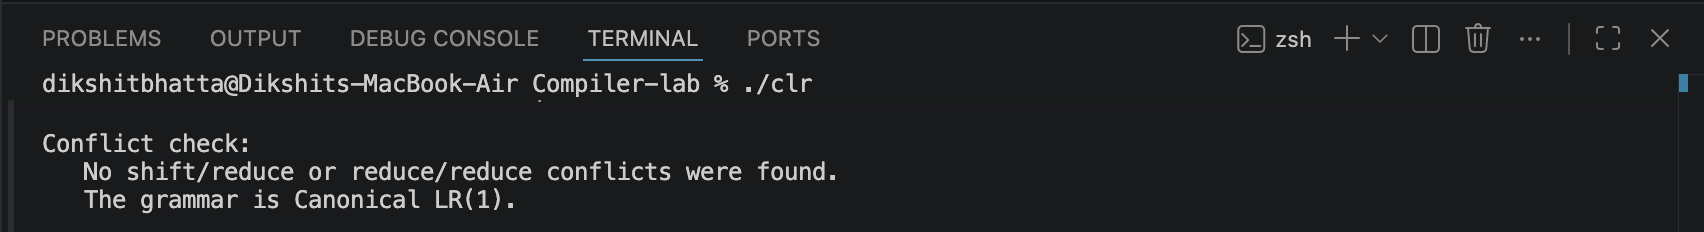
\includegraphics[width=\textwidth]{output/output6.png}
\caption{Conflict check: no shift/reduce or reduce/reduce conflicts.}
\end{figure}

Every cell of the parsing table (Figure~\ref{fig:ptable}) holds at most one
entry, so the table is \textbf{conflict-free}. The critical cell is row $I_2$: it carries \texttt{s6}
under \texttt{=} and \texttt{r5} under \texttt{\$}---two \emph{different}
columns. Because the canonical method kept the look-ahead \texttt{\$} (and not
\texttt{=}) on the item $[R \rightarrow L \bullet,\ \$]$, no shift/reduce
conflict appears, even though $\texttt{=} \in \mathrm{FOLLOW}(R)$ would have
forced one under SLR(1). This is the result the project set out to demonstrate.

\section{Validation on Test Strings}

\subsection{String \texttt{id = *id} (accepted)}
\begin{figure}[H]
\centering
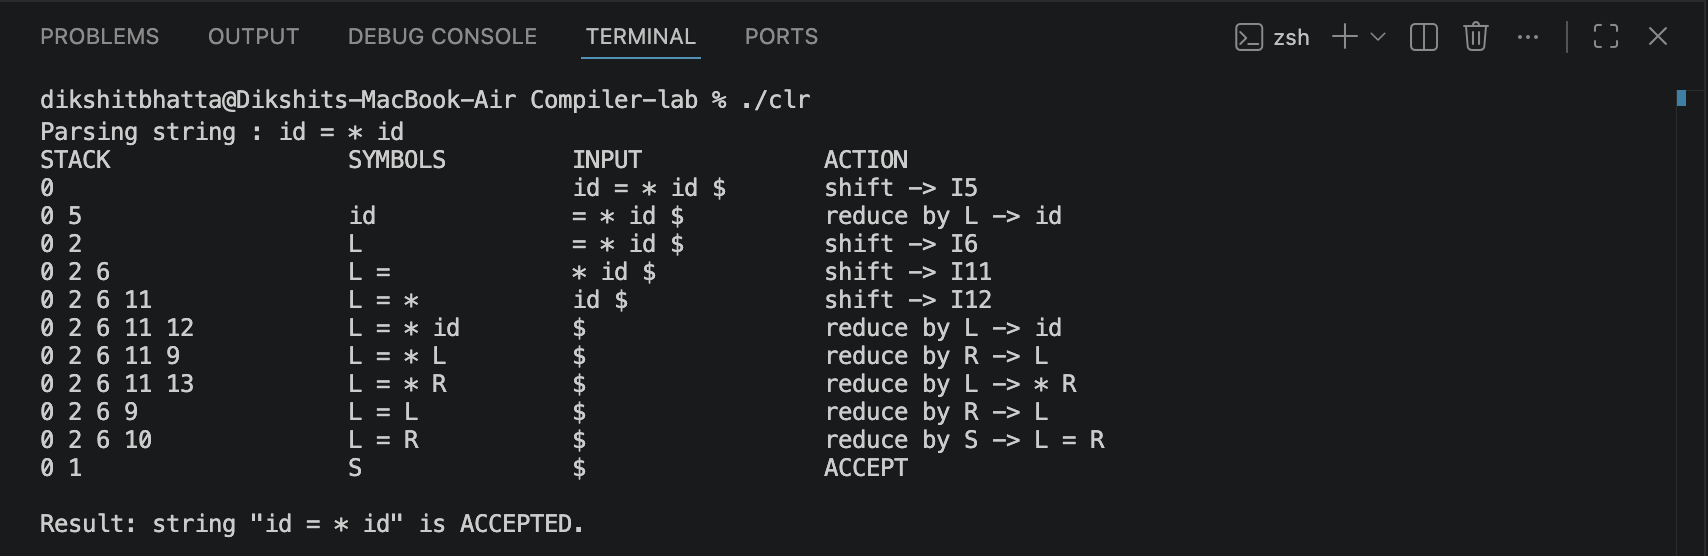
\includegraphics[width=\textwidth]{output/output7.png}
\caption{Parse trace for \texttt{id = *id}: the string is accepted.}
\end{figure}

\subsection{String \texttt{id = id * id} (rejected)}
The literal three-operand string is not in the language, because \texttt{*} is a
prefix operator and cannot appear between two \texttt{id}s. The parser detects
the error exactly where the second \texttt{id} is followed by \texttt{*}:
\begin{figure}[H]
\centering
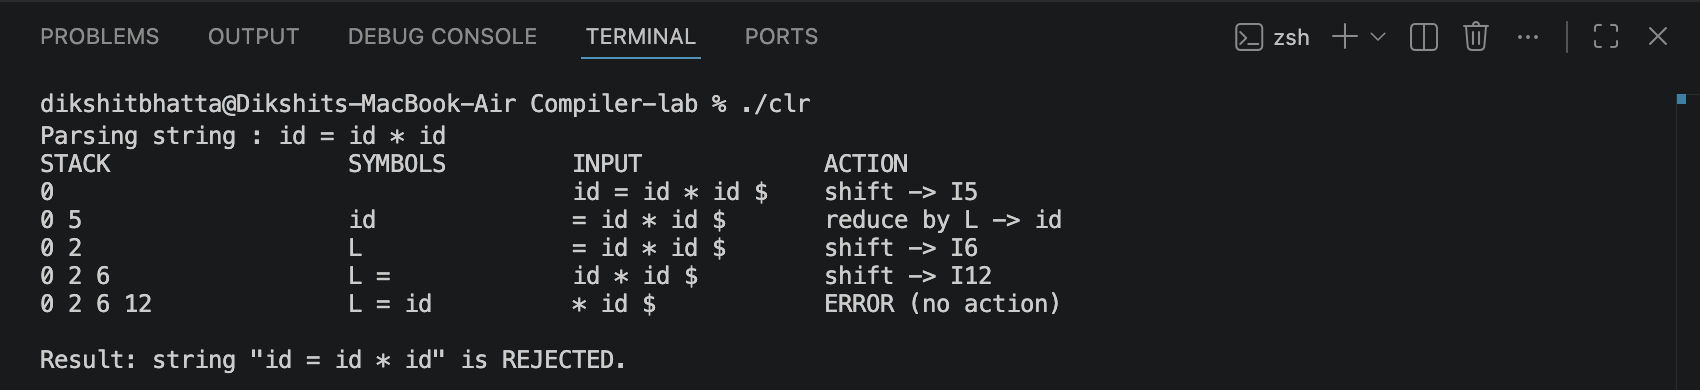
\includegraphics[width=\textwidth]{output/output8.png}
\caption{Parse trace for \texttt{id = id * id}: the string is rejected.}
\end{figure}
State $I_{12}$ contains only $[L \rightarrow \texttt{id} \bullet,\ \$]$, so the
only legal next symbol is \texttt{\$}; seeing \texttt{*} is a syntax error. The
parser thus accepts exactly the strings the grammar generates.

%==============================================================================
\chapter{Conclusion and Recommendation}
%==============================================================================

\section{Conclusion}
This project implemented a complete canonical LR(1) parser in C++ for the
augmented grammar $S' \rightarrow S$, $S \rightarrow L = R \mid R$,
$L \rightarrow {*}R \mid \texttt{id}$, $R \rightarrow L$. The program builds the
FIRST sets, the 14-state canonical collection of LR(1) item sets, the goto
automaton, and the \texttt{ACTION}/\texttt{GOTO} parsing table, and it
automatically checks for conflicts. The central result is that the table has
\textbf{no shift/reduce or reduce/reduce conflict}, even though the same grammar
is \emph{not} SLR(1)---the difference being the exact one-symbol look-ahead that
canonical LR(1) carries on each item, which keeps the shift on \texttt{=} and
the reduction on \texttt{\$} in separate cells of state $I_2$. The table was
validated by parsing \texttt{id = *id}, which is accepted with a full reverse
rightmost derivation, while the malformed \texttt{id = id * id} is correctly
rejected.

\section{Future Enhancement}
\begin{itemize}
  \item \textbf{Generic input:} read an arbitrary grammar and string from a file or web form, rather than the hard-coded grammar.
  \item \textbf{LALR(1) construction:} merge LR(1) states with identical cores to show the size reduction (14 states $\rightarrow$ fewer) and discuss the look-ahead trade-off.
  \item \textbf{Error recovery:} replace the simple ``reject'' with panic-mode or phrase-level recovery and informative diagnostics.
  \item \textbf{Visualization:} render the goto automaton and animate the stack during parsing through a web interface.
\end{itemize}

%==============================================================================
\chapter{References}
%==============================================================================
\begin{enumerate}
  \item A. V. Aho, M. S. Lam, R. Sethi, and J. D. Ullman, \emph{Compilers: Principles, Techniques, and Tools}, 2nd ed. Boston, MA: Pearson/Addison-Wesley, 2007.
  \item K. C. Louden, \emph{Compiler Construction: Principles and Practice}. Boston, MA: PWS Publishing, 1997.
  \item GeeksforGeeks, ``Canonical LR / CLR(1) parser,'' \url{https://www.geeksforgeeks.org/clr-1-parser-introduction/}.
  \item Javatpoint, ``LR Parser,'' \url{https://www.javatpoint.com/lr-parser}.
  \item Wikipedia contributors, ``Canonical LR parser,'' \emph{Wikipedia}, \url{https://en.wikipedia.org/wiki/Canonical_LR_parser}.
\end{enumerate}

%==============================================================================
\appendix
\chapter{Complete Source Code}
\label{app:code}
The complete C++ implementation (\texttt{canonical\_lr\_parser.cpp}), captured
directly from Visual Studio Code, is reproduced below.

\begin{center}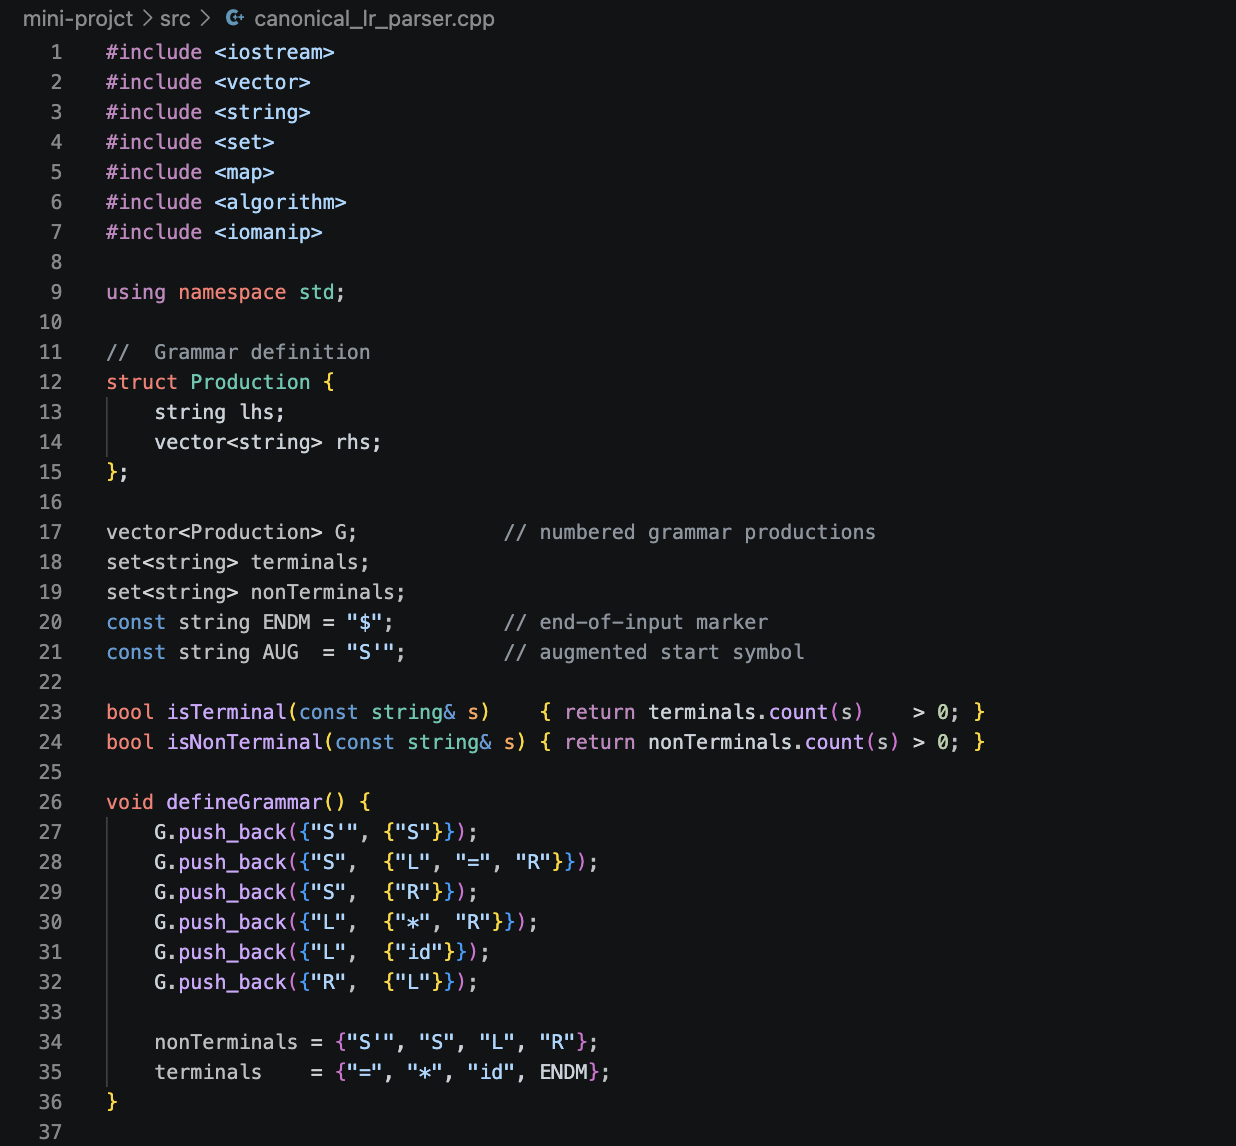
\includegraphics[width=\textwidth]{code/code1.png}\end{center}
\begin{center}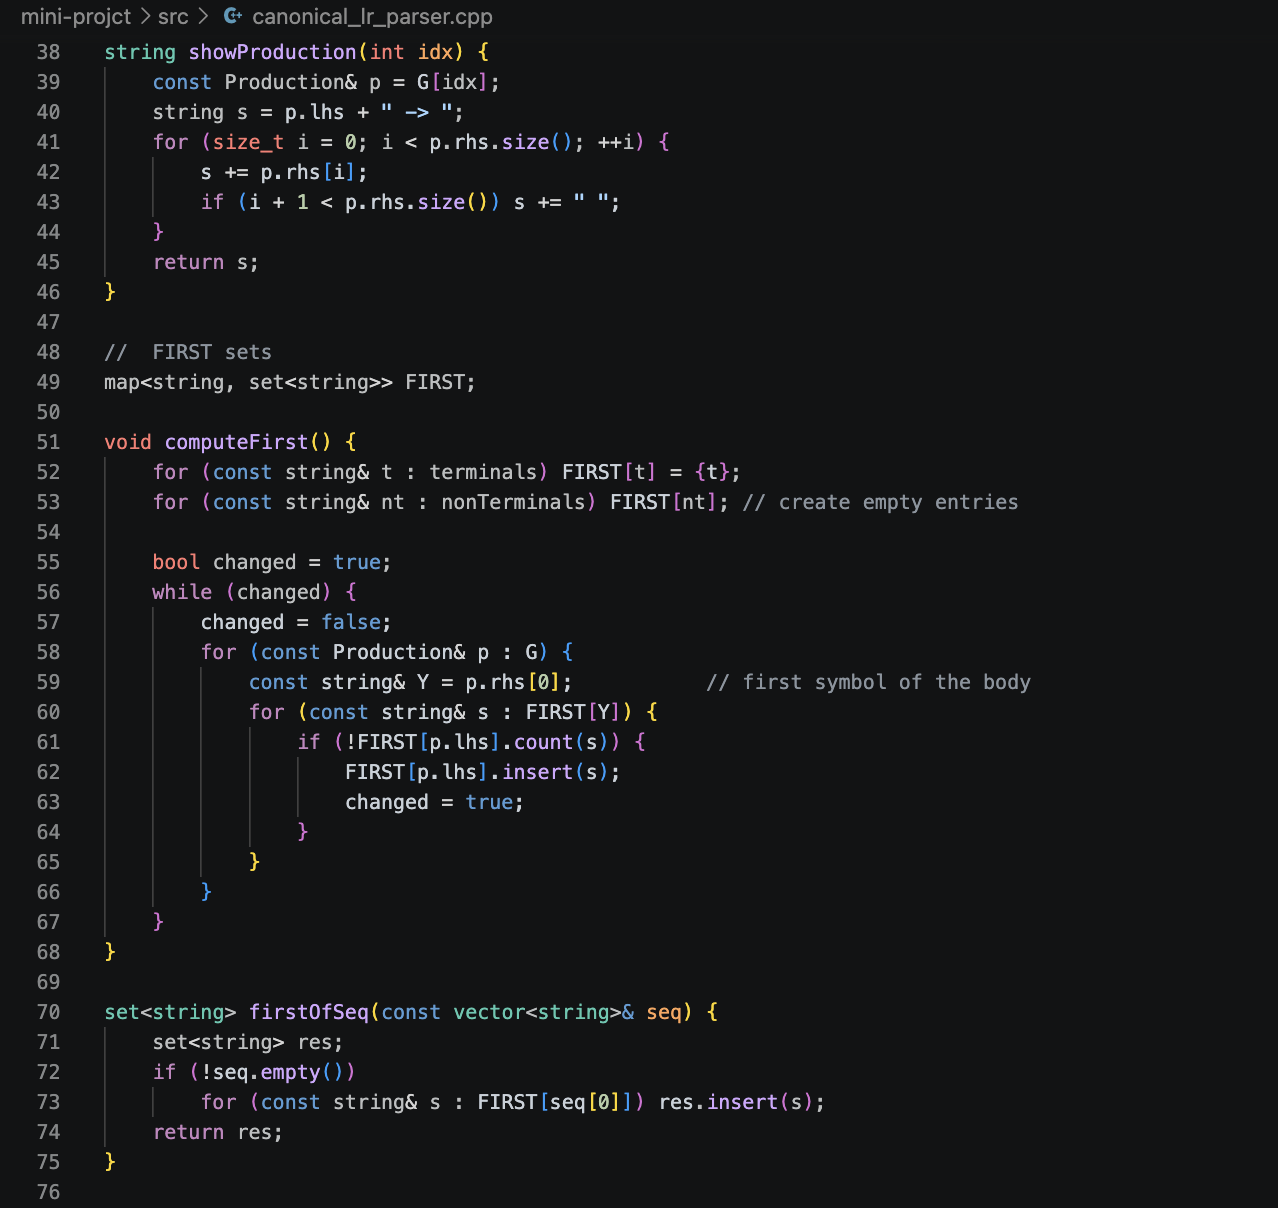
\includegraphics[width=\textwidth]{code/code2.png}\end{center}
\begin{center}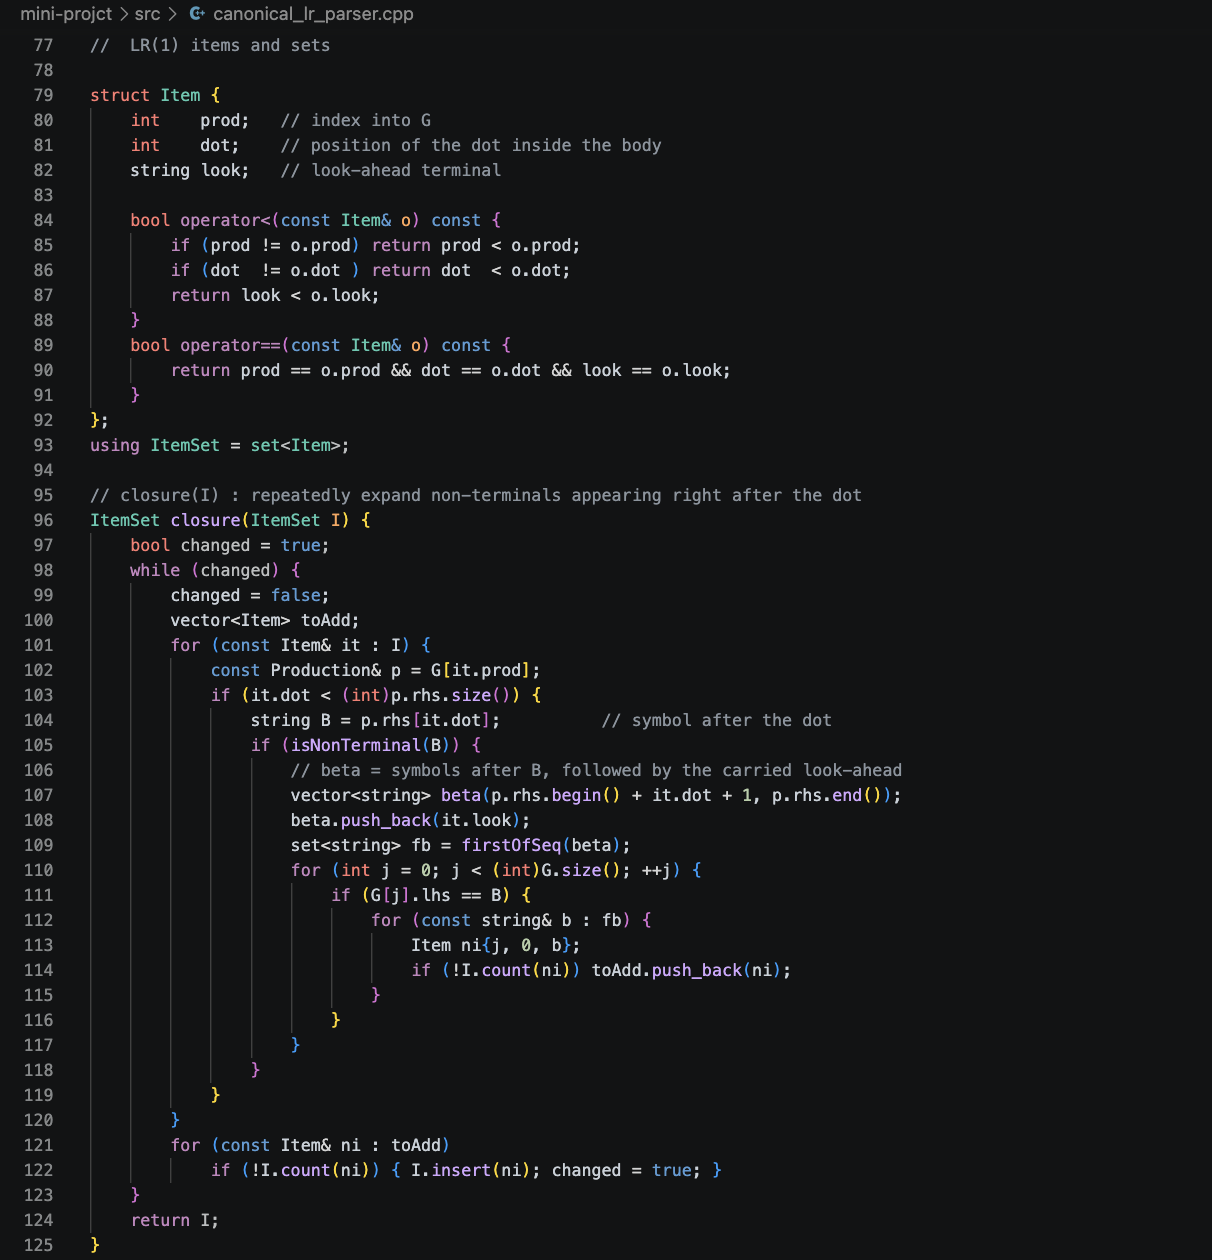
\includegraphics[width=\textwidth]{code/code3.png}\end{center}
\begin{center}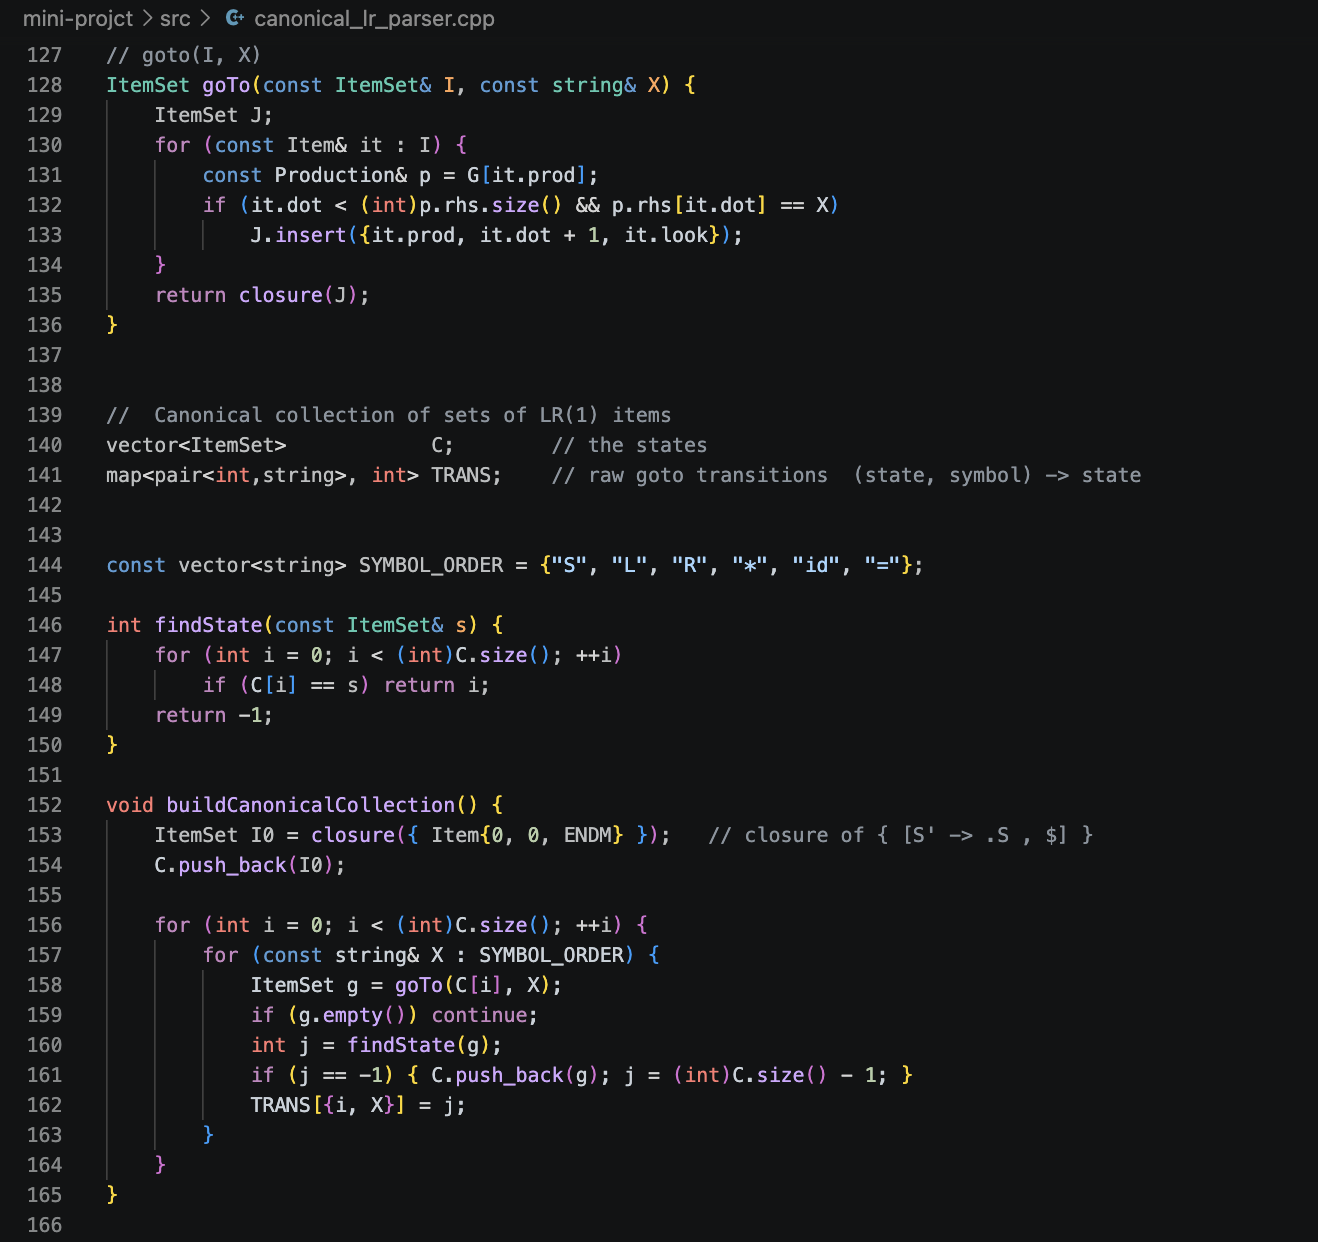
\includegraphics[width=\textwidth]{code/code4.png}\end{center}
\begin{center}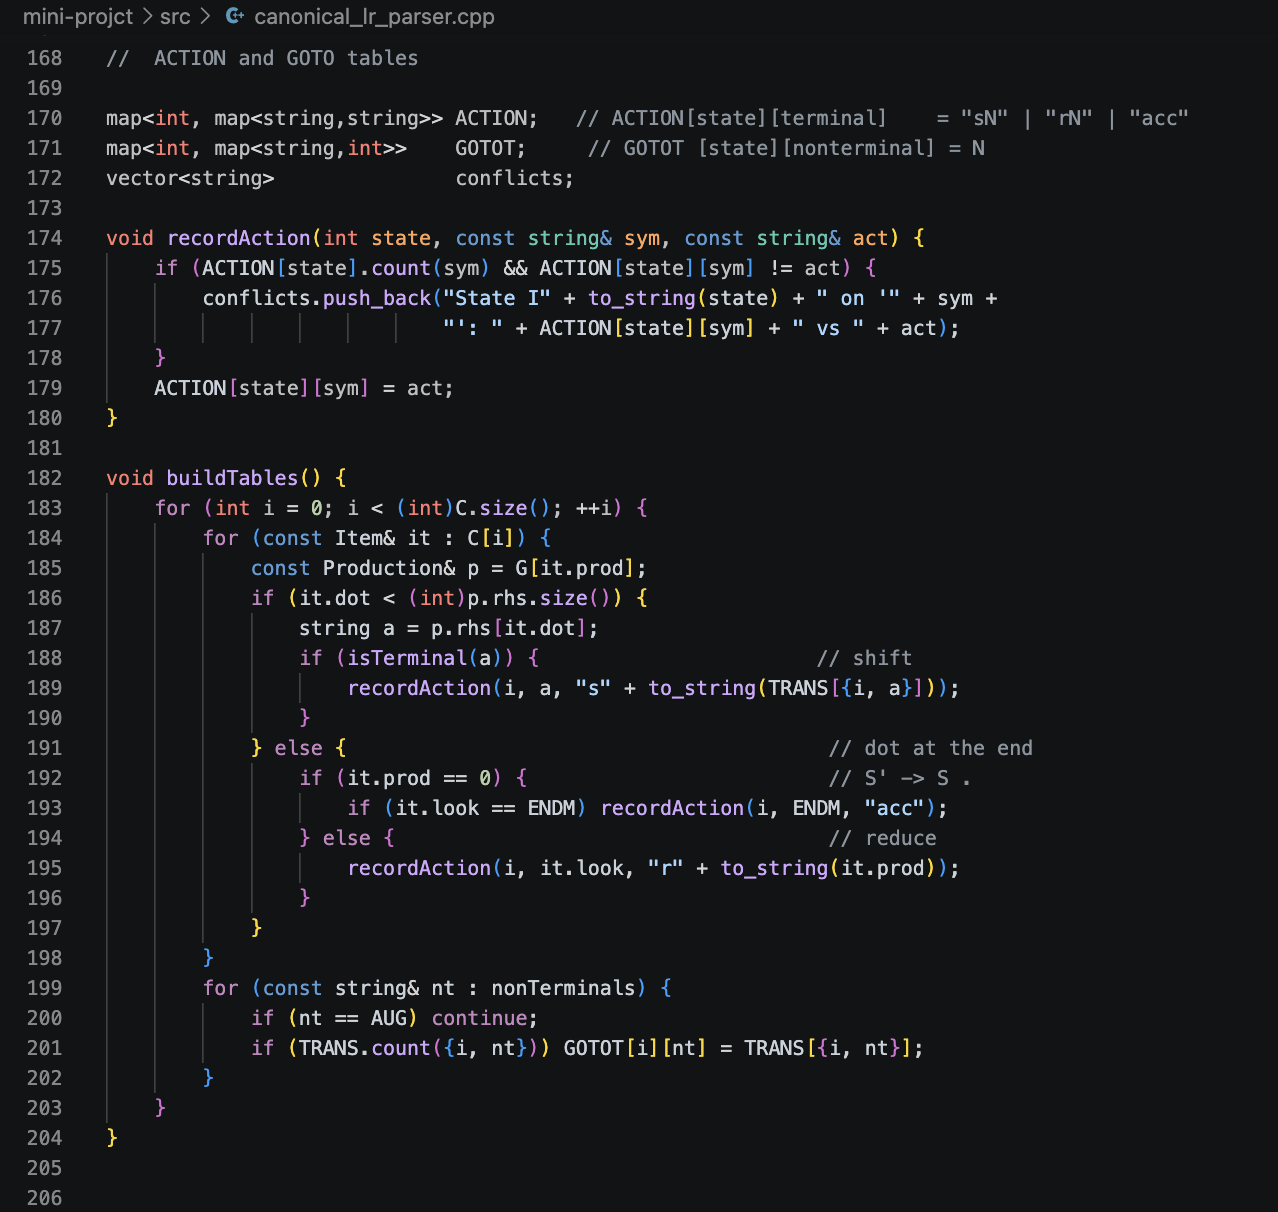
\includegraphics[width=\textwidth]{code/code5.png}\end{center}
\begin{center}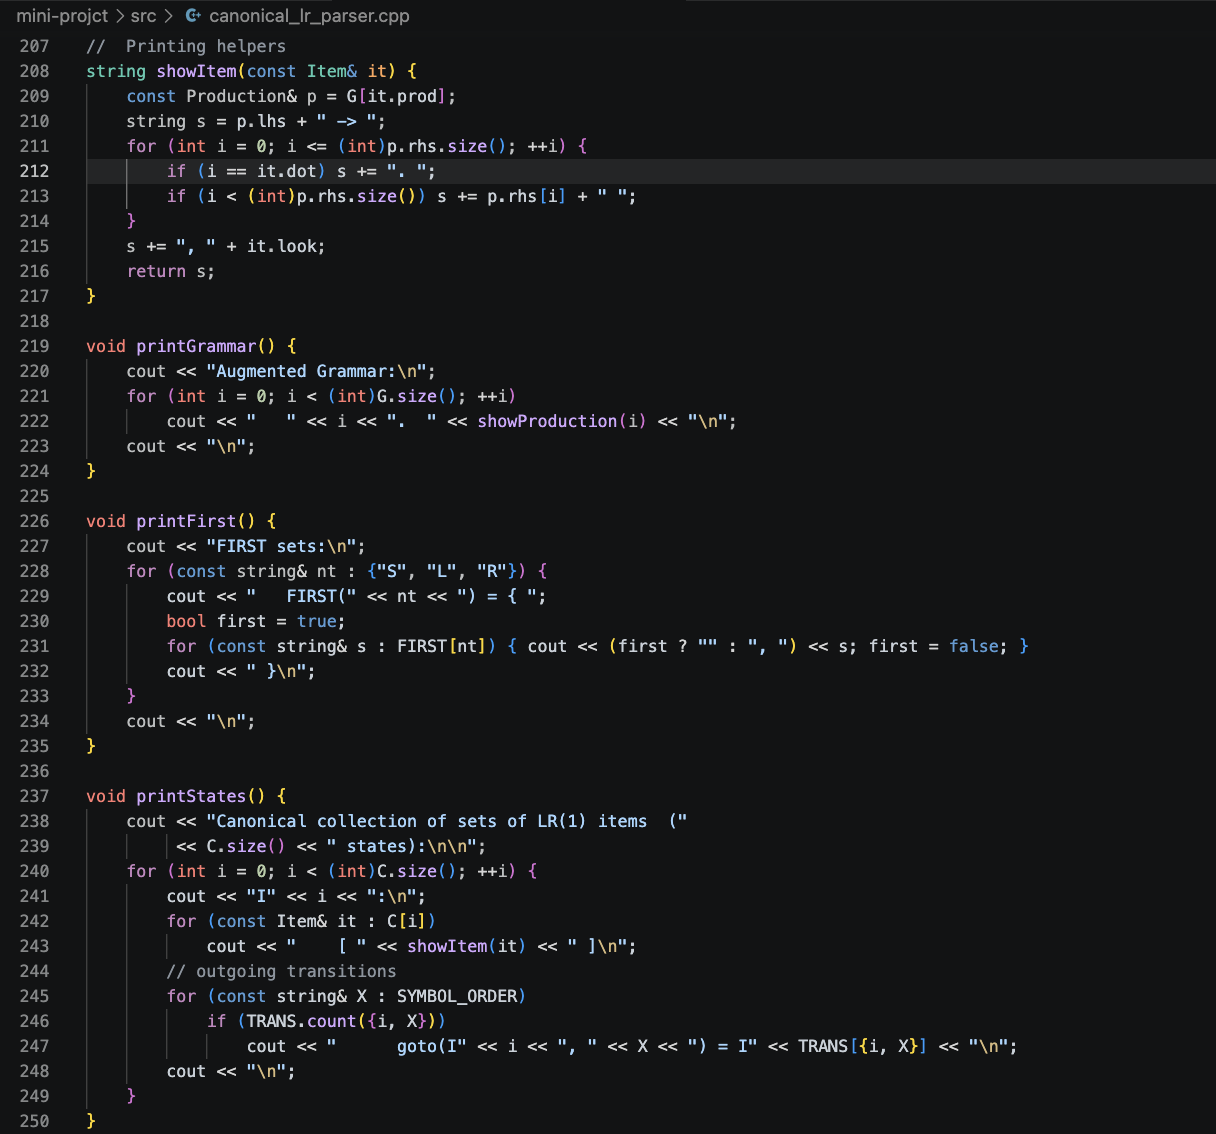
\includegraphics[width=\textwidth]{code/code6.png}\end{center}
\begin{center}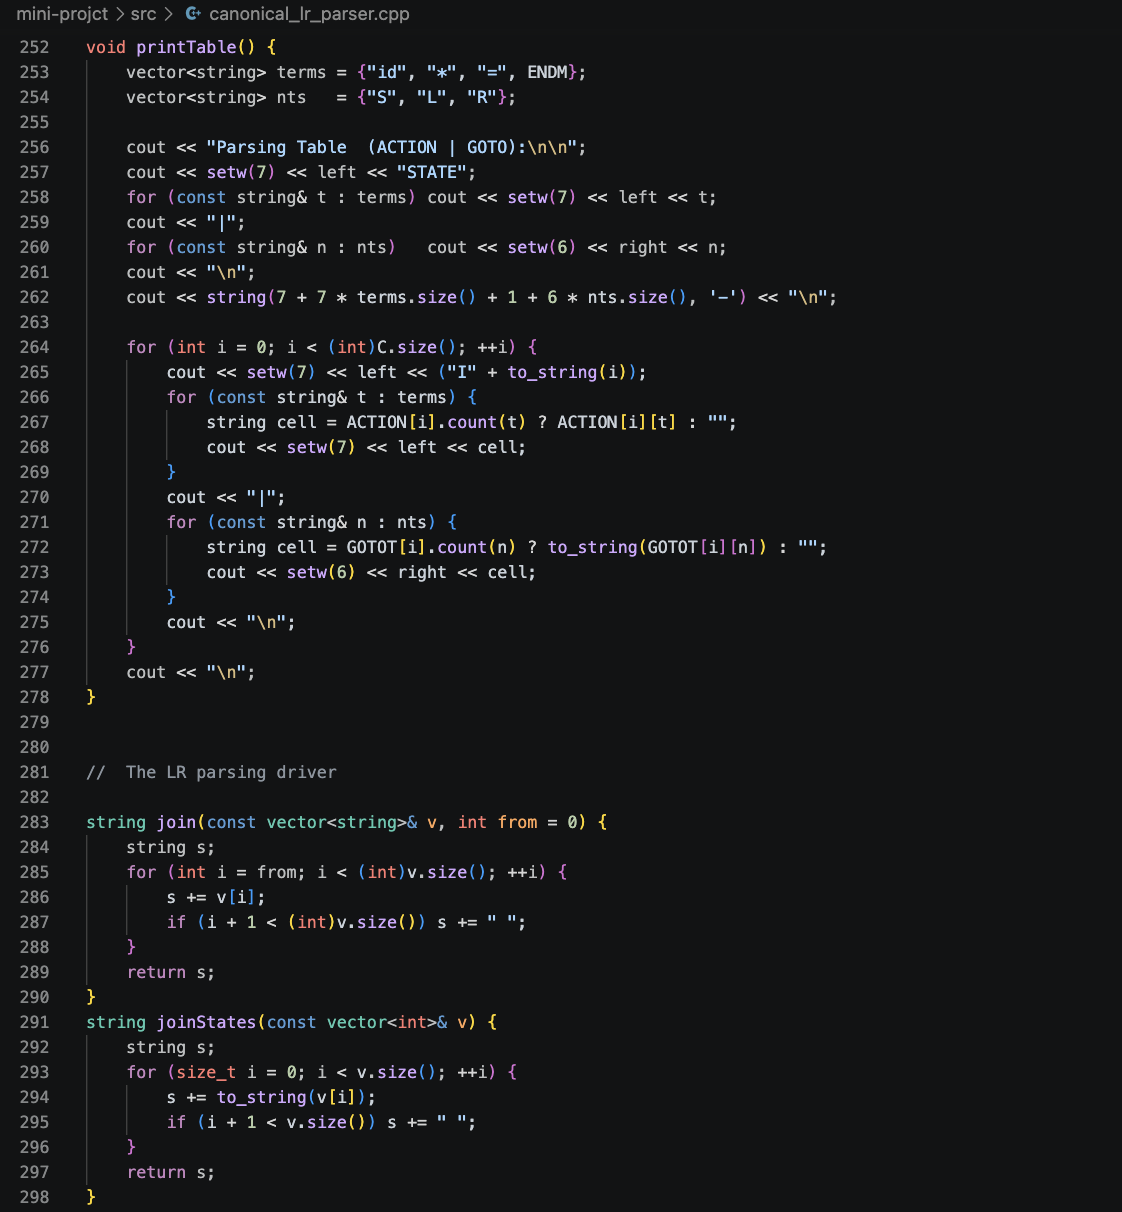
\includegraphics[width=\textwidth]{code/code7.png}\end{center}
\begin{center}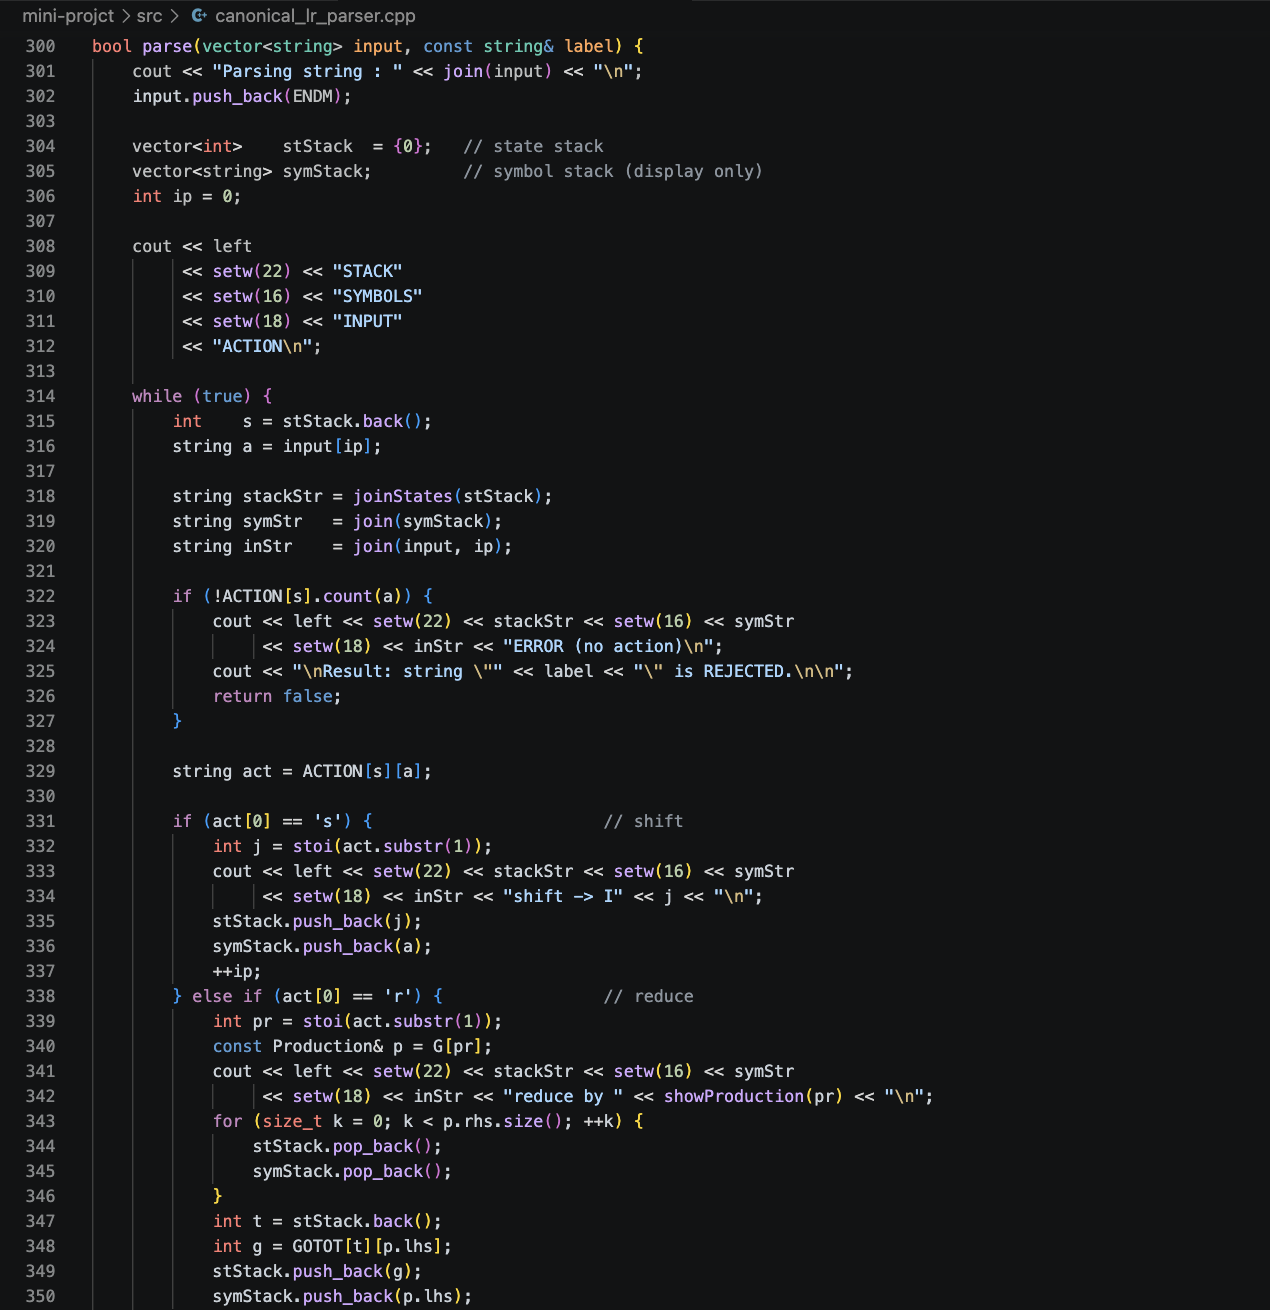
\includegraphics[width=\textwidth]{code/code8.png}\end{center}
\begin{center}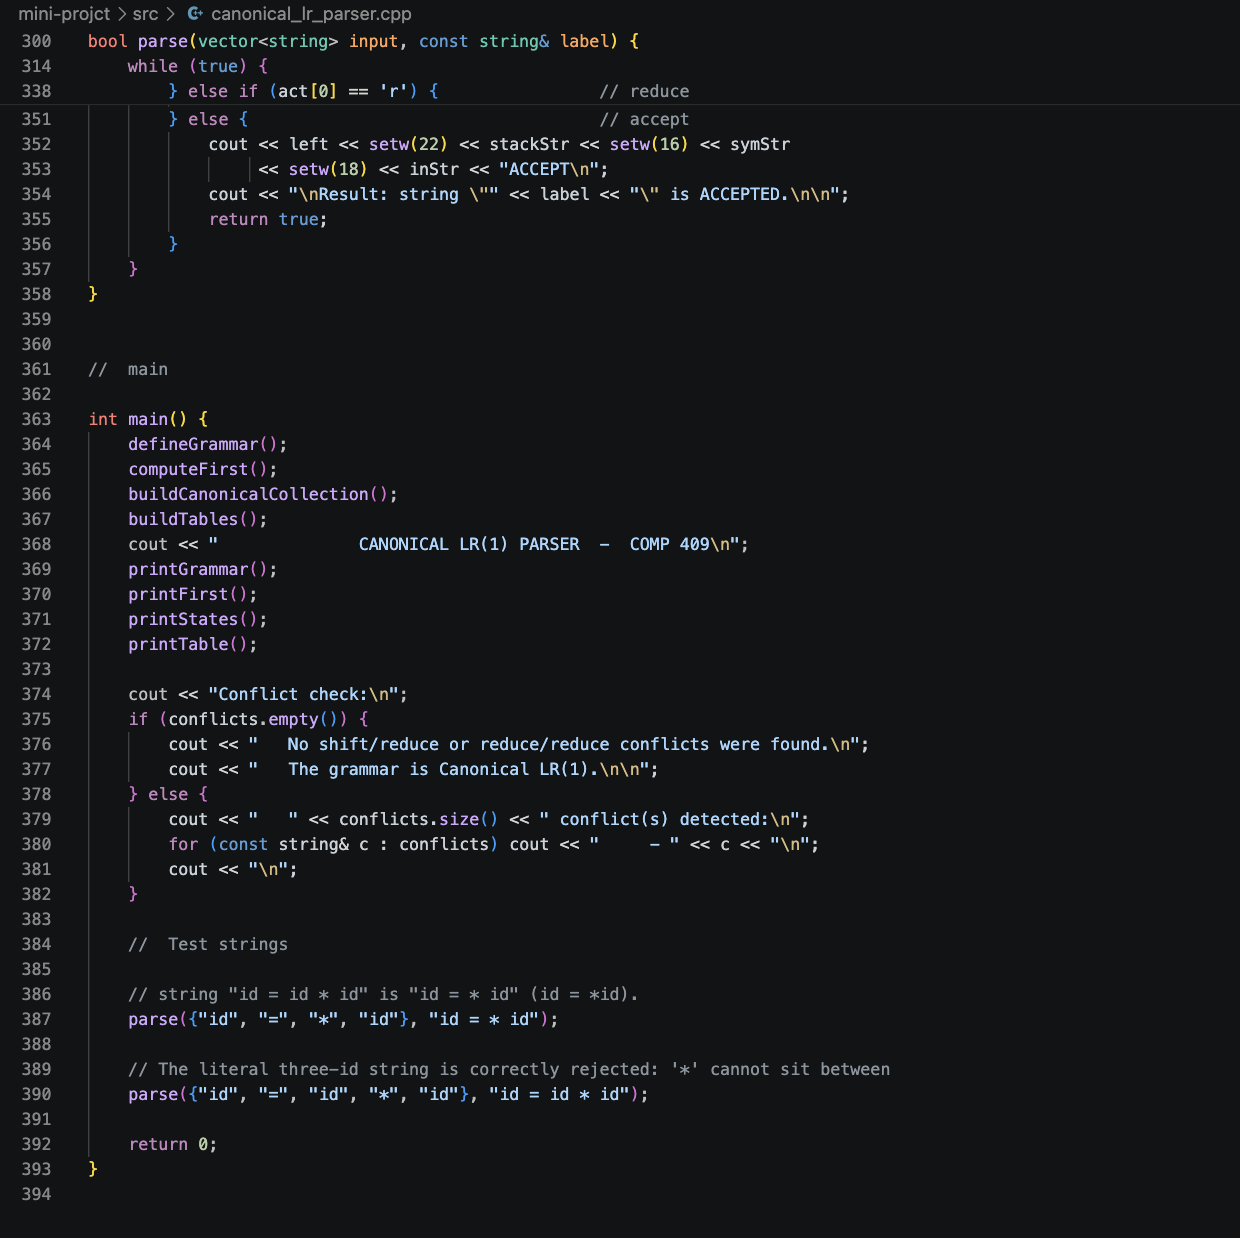
\includegraphics[width=\textwidth]{code/code9.png}\end{center}

\end{document}
